%TC:ignore - ignoriert die folgnden Wörter beim Wordcount in Overleaf 
%-----------------------------------
% Define document and include general packages
%-----------------------------------
% Tabellen- und Abbildungsverzeichnis stehen normalerweise nicht im
% Inhaltsverzeichnis. Gleiches gilt für das Abkürzungsverzeichnis (siehe unten).
% Manche Dozenten bemängeln das. Die Optionen 'listof=totoc,bibliography=totoc'
% geben das Tabellen- und Abbildungsverzeichnis im Inhaltsverzeichnis (toc=Table
% of Content) aus.
% Da es aber verschiedene Regelungen je nach Dozent geben kann, werden hier
% beide Varianten dargestellt.
\documentclass[12pt,oneside,titlepage,listof=totoc,bibliography=totoc]{scrartcl}
%\documentclass[12pt,oneside,titlepage]{scrartcl}

%-----------------------------------
% Dokumentensprache
%-----------------------------------
\def\FOMEN{}% Auskommentieren um die Dokumentensprache auf englisch zu ändern
\newif\ifde
\newif\ifen

%-----------------------------------
% Meta informationen
%-----------------------------------
%-----------------------------------
% Meta Informationen zur Arbeit
%-----------------------------------

% Autor
\newcommand{\myAutor}{Karl Wedrich}

% Adresse
\newcommand{\myAdresse}{Dorothea-Bernstein-Weg 3 \\ \> \> \> 22081 Hamburg}

% Titel der Arbeit
\newcommand{\myTitel}{Avoiding Software Decay in Military Software Development}

% Betreuer
\newcommand{\myBetreuer}{Prof. Dr. Ulrich Schüler}

% Lehrveranstaltung
\newcommand{\myLehrveranstaltung}{Modul Nr. 1}

% Matrikelnummer
\newcommand{\myMatrikelNr}{597615}

% Ort
\newcommand{\myOrt}{Hamburg}

% Datum der Abgabe
\newcommand{\myAbgabeDatum}{\today}

% Semesterzahl
\newcommand{\mySemesterZahl}{7}

% Name der Hochschule
\newcommand{\myHochschulName}{FOM Hochschule für Oekonomie \& Management}

% Standort der Hochschule
\newcommand{\myHochschulStandort}{Hamburg}

% Studiengang
\newcommand{\myStudiengang}{Wirtschaftsinformatik}

% Art der Arbeit
\newcommand{\myThesisArt}{Bachelor Thesis}

% Zu erlangender akademische Grad
\newcommand{\myAkademischerGrad}{Bachelor of Science (B.Sc.)}

% Firma
\newcommand{\myFirma}{Telekom Deutschland GmbH}

% Definition der Sprache
\ifdefined\FOMEN
%Englisch
\entrue
\usepackage[english]{babel}
\else
%Deutsch
\detrue
\usepackage[ngerman]{babel}
\fi


\newcommand{\langde}[1]{%
   \ifde\selectlanguage{ngerman}#1\fi}
\newcommand{\langen}[1]{%
   \ifen\selectlanguage{english}#1\fi}
\usepackage[utf8]{luainputenc}
\langde{\usepackage[babel,german=quotes]{csquotes}}
\langen{\usepackage[babel,english=british]{csquotes}}
\ifde\usepackage[ngerman]{babel}\fi
\usepackage[T1]{fontenc}
\usepackage{fancyhdr}
\usepackage{fancybox}
\usepackage[a4paper, left=4cm, right=2cm, top=4cm, bottom=2cm]{geometry}
\usepackage{graphicx}
\usepackage{colortbl}
\usepackage[capposition=top]{floatrow}
\usepackage{array}
\usepackage{float}      %Positionierung von Abb. und Tabellen mit [H] erzwingen
\usepackage{footnote}
% Darstellung der Beschriftung von Tabellen und Abbildungen (Leitfaden S. 44)
% singlelinecheck=false: macht die Caption linksbündig (statt zentriert)
% labelfont auf fett: (Tabelle x.y:, Abbildung: x.y)
% font auf fett: eigentliche Bezeichnung der Abbildung oder Tabelle
% Fettschrift laut Leitfaden 2018 S. 45
\usepackage[singlelinecheck=false, labelfont=bf, font=bf]{caption}
\usepackage{caption}
\usepackage{enumitem}
\usepackage{amssymb}
\usepackage{mathptmx}
%\usepackage{minted} %Kann für schöneres Syntax Highlighting genutzt werden. ACHTUNG: Python muss installiert sein.
\usepackage[scaled=0.9]{helvet} % Behebt, zusammen mit Package courier, pixelige Überschriften. Ist, zusammen mit mathptx, dem times-Package vorzuziehen. Details: https://latex-kurs.de/fragen/schriftarten/Times_New_Roman.html
\usepackage{courier}
\usepackage{amsmath}
\usepackage[table]{xcolor}
\usepackage{marvosym}			% Verwendung von Symbolen, z.B. perfektes Eurozeichen

\renewcommand\familydefault{\sfdefault}
\usepackage{ragged2e}

% Mehrere Fussnoten nacheinander mit Komma separiert
\usepackage[hang,multiple]{footmisc}
\setlength{\footnotemargin}{1em}

% todo Aufgaben als Kommentare verfassen für verschiedene Editoren
\usepackage{todonotes}

% Verhindert, dass nur eine Zeile auf der nächsten Seite steht
\setlength{\marginparwidth}{2cm}
\usepackage[all]{nowidow}

%-----------------------------------
% Farbdefinitionen
%-----------------------------------
\definecolor{darkblack}{rgb}{0,0,0}
\definecolor{dunkelgrau}{rgb}{0.8,0.8,0.8}
\definecolor{hellgrau}{rgb}{0.0,0.7,0.99}
\definecolor{mauve}{rgb}{0.58,0,0.82}
\definecolor{dkgreen}{rgb}{0,0.6,0}

%-----------------------------------
% Pakete für Tabellen
%-----------------------------------
\usepackage{epstopdf}
\usepackage{nicefrac} % Brüche
\usepackage{multirow}
\usepackage{rotating} % vertikal schreiben
\usepackage{mdwlist}
\usepackage{tabularx}% für Breitenangabe

%-----------------------------------
% sauber formatierter Quelltext
%-----------------------------------
\usepackage{listings}
% JavaScript als Sprache definieren:
\lstdefinelanguage{JavaScript}{
	keywords={break, super, case, extends, switch, catch, finally, for, const, function, try, continue, if, typeof, debugger, var, default, in, void, delete, instanceof, while, do, new, with, else, return, yield, enum, let, await},
	keywordstyle=\color{blue}\bfseries,
	ndkeywords={class, export, boolean, throw, implements, import, this, interface, package, private, protected, public, static},
	ndkeywordstyle=\color{darkgray}\bfseries,
	identifierstyle=\color{black},
	sensitive=false,
	comment=[l]{//},
	morecomment=[s]{/*}{*/},
	commentstyle=\color{purple}\ttfamily,
	stringstyle=\color{red}\ttfamily,
	morestring=[b]',
	morestring=[b]"
}

\lstset{
	%language=JavaScript,
	numbers=left,
	numberstyle=\tiny,
	numbersep=5pt,
	breaklines=true,
	showstringspaces=false,
	frame=l ,
	xleftmargin=5pt,
	xrightmargin=5pt,
	basicstyle=\ttfamily\scriptsize,
	stepnumber=1,
	keywordstyle=\color{blue},          % keyword style
  	commentstyle=\color{dkgreen},       % comment style
  	stringstyle=\color{mauve}         % string literal style
}

%-----------------------------------
%Literaturverzeichnis Einstellungen
%-----------------------------------

% Biblatex

\usepackage{url}
\urlstyle{same}
\newcommand{\citationstyle}{fom_2018} % Mögliche Werte: ieee, fom_2018, fom_alt
% Laden des entsprechenden Zitationsstils basierend auf der Variable \citationstyle
\ifthenelse{\equal{\citationstyle}{ieee}}{
    % Einstellungen für IEEE-Zitationsstil
	\usepackage[
		backend=biber,
		style=ieee,
		maxcitenames=3,	% mindestens 3 Namen ausgeben bevor et. al. kommt
		maxbibnames=999,
		date=iso,
		seconds=true, %werden nicht verwendet, so werden aber Warnungen unterdrückt.
		urldate=iso,
		dashed=false,
		autocite=inline,
		useprefix=true, % 'von' im Namen beachten (beim Anzeigen)
		mincrossrefs = 1
	]{biblatex}%iso dateformat für YYYY-MM-DD
    % et al. anstatt u. a. bei mehr als drei Autoren.
    \DefineBibliographyStrings{ngerman}{
        andothers = {{et\,al\adddot}},
    }
    \DefineBibliographyStrings{english}{
        andothers = {{et\,al\adddot}},
    }
}{
    \ifthenelse{\equal{\citationstyle}{fom_2018}}{
        % Einstellungen für Neuer Leitfaden (2018)
		\usepackage[
			backend=biber,
			style=ext-authoryear-ibid, % Auskommentieren und nächste Zeile einkommentieren, falls "Ebd." (ebenda) nicht für sich-wiederholende Fussnoten genutzt werden soll.
			%style=ext-authoryear,
			maxcitenames=3,	% mindestens 3 Namen ausgeben bevor et. al. kommt
			maxbibnames=999,
			mergedate=false,
			date=iso,
			seconds=true, %werden nicht verwendet, so werden aber Warnungen unterdrückt.
			urldate=iso,
			innamebeforetitle,
			dashed=false,
			autocite=footnote,
			doi=false,
			useprefix=true, % 'von' im Namen beachten (beim Anzeigen)
			mincrossrefs = 1
		]{biblatex}%iso dateformat für YYYY-MM-DD
        %weitere Anpassungen für BibLaTex
        \usepackage{xpatch}

\setlength\bibhang{1cm}

%%% Weitere Optionen
%\boolitem[false]{citexref} %Wenn incollection, inbook, inproceedings genutzt wird nicht den zugehörigen parent auch in Literaturverzeichnis aufnehmen

%Aufräumen die Felder werden laut Leitfaden nicht benötigt.
\AtEveryBibitem{%
\ifentrytype{book}{
    \clearfield{issn}%
    \clearfield{doi}%
    \clearfield{isbn}%
    \clearfield{url}
    \clearfield{eprint}
}{}
\ifentrytype{collection}{
  \clearfield{issn}%
  \clearfield{doi}%
  \clearfield{isbn}%
  \clearfield{url}
  \clearfield{eprint}
}{}
\ifentrytype{incollection}{
  \clearfield{issn}%
  \clearfield{doi}%
  \clearfield{isbn}%
  \clearfield{url}
  \clearfield{eprint}
}{}
\ifentrytype{article}{
  \clearfield{issn}%
  \clearfield{doi}%
  \clearfield{isbn}%
  \clearfield{url}
  \clearfield{eprint}
}{}
\ifentrytype{inproceedings}{
  \clearfield{issn}%
  \clearfield{doi}%
  \clearfield{isbn}%
  \clearfield{url}
  \clearfield{eprint}
}{}
}

\renewcommand*{\finentrypunct}{}%Kein Punkt am ende des Literaturverzeichnisses

\renewcommand*{\newunitpunct}{\addcomma\space}
\DeclareDelimFormat[bib,biblist]{nametitledelim}{\addcolon\space}
\DeclareDelimFormat{titleyeardelim}{\newunitpunct}
%Namen kursiv schreiben
\renewcommand*{\mkbibnamefamily}{\mkbibemph}
\renewcommand*{\mkbibnamegiven}{\mkbibemph}
\renewcommand*{\mkbibnamesuffix}{\mkbibemph}
\renewcommand*{\mkbibnameprefix}{\mkbibemph}

% Die Trennung mehrerer Autorennamen erfolgt durch Kommata.
% siehe Beispiele im Leitfaden S. 16
% Die folgende Zeile würde mit Semikolon trennen
%\DeclareDelimFormat{multinamedelim}{\addsemicolon\addspace}

%Delimiter für mehrere und letzten Namen gleich setzen
\DeclareDelimAlias{finalnamedelim}{multinamedelim}

\DeclareNameAlias{default}{family-given}
\DeclareNameAlias{sortname}{default}  %Nach Namen sortieren


\DeclareFieldFormat{editortype}{\mkbibparens{#1}}
\DeclareDelimFormat{editortypedelim}{\addspace}
\DeclareFieldFormat{translatortype}{\mkbibparens{#1}}
\DeclareDelimFormat{translatortypedelim}{\addspace}
\DeclareDelimFormat[bib,biblist]{innametitledelim}{\addcomma\space}

\DeclareFieldFormat*{citetitle}{#1}
\DeclareFieldFormat*{title}{#1}
\DeclareFieldFormat*{booktitle}{#1}
\DeclareFieldFormat*{journaltitle}{#1}

\xpatchbibdriver{online}
  {\usebibmacro{organization+location+date}\newunit\newblock}
  {}
  {}{}

\DeclareFieldFormat[online]{date}{\mkbibparens{#1}}
\DeclareFieldFormat{urltime}{\addspace #1\addspace \langde{Uhr}\langen{MEZ}}
\DeclareFieldFormat{urldate}{%urltime zu urldate hinzufügen
  [\langde{Zugriff}\langen{Access}\addcolon\addspace
  #1\printfield{urltime}]
}
\DeclareFieldFormat[online]{url}{<\url{#1}>}
\renewbibmacro*{url+urldate}{%
  \usebibmacro{url}%
  \ifentrytype{online}
    {\setunit*{\addspace}%
     \iffieldundef{year}
       {\printtext[date]{keine Datumsangabe }}
       {\usebibmacro{date}}%
       \setunit*{\addspace}%
       \usebibmacro{urldate}}%
    {}%
  }

%Verhindern, dass bei mehreren Quellen des gleichen Autors im gleichen Jahr
%Buchstaben nach der Jahreszahl angezeigt werden wenn sich das Keyword in shorttitle unterscheidet.
\DeclareExtradate{
  \scope{
    \field{labelyear}
    \field{year}
    }
    \scope{
      \field{shorttitle}
     }
}

%% Anzeige des Jahres nach dem Stichwort (shorttitle) im Literaturverzeichnis
%% Wenn das Jahr bei Online-Quellen nicht explizit angegeben wurde, wird nach
%% dem Stichwort 'o. J.' ausgegeben. Nach der URL steht dann 'keine
%% Datumsangabe'. Ist das Jahr definiert, wird es an beiden Stellen ausgegeben.
%% Das Zugriffsdatum (urldate) spielt hier keine Rolle.
%% Für Nicht-Online-Quellen wird nichts geändert.
\renewbibmacro*{date+extradate}{%
  \printtext[parens]{%
    \printfield{shorttitle}%
    \setunit{\printdelim{titleyeardelim}}%
    \ifentrytype{online}
       {\setunit*{\addspace\addcomma\addspace}%
         \iffieldundef{year}
           {\bibstring{nodate}}
       {\printlabeldateextra}}%
       {\printlabeldateextra}}}

%% Anzeige des Jahres nach dem Stichwort (shorttitle) in der Fussnote
%% das Stichwort hat der Aufrufer hier schon ausgegeben.
%% siehe auch Kommentar zu: \renewbibmacro*{date+extradate}
\renewbibmacro*{cite:labeldate+extradate}{%
    \ifentrytype{online}
       {\setunit*{\addspace\addcomma\addspace}%
         \iffieldundef{year}
           {\bibstring{nodate}}
       {\printlabeldateextra}}%
       {\printlabeldateextra}}


\DefineBibliographyStrings{german}{
  nodate    = {{}o.\adddot\addspace J\adddot},
  andothers = {et\addabbrvspace al\adddot}
}
\DefineBibliographyStrings{english}{
  nodate    = {{}n.\adddot\addspace d\adddot},
  andothers = {et\addabbrvspace al\adddot}
}
\DeclareSourcemap{
  \maps[datatype=bibtex]{
    \map{
      \step[notfield=translator, final]
      \step[notfield=editor, final]
      \step[fieldset=author, fieldvalue={{{\langde{o\noexpand\adddot\addspace V\noexpand\adddot}\langen{Anon}}}}]
    }
    \map{
      \pernottype{online}
      \step[fieldset=location, fieldvalue={\langde{o\noexpand\adddot\addspace O\noexpand\adddot}\langen{s\noexpand\adddot I\noexpand\adddot}}]
    }
  }
}

\renewbibmacro*{cite}{%
  \iffieldundef{shorthand}
    {\ifthenelse{\ifnameundef{labelname}\OR\iffieldundef{labelyear}}
       {\usebibmacro{cite:label}%
        \setunit{\printdelim{nonametitledelim}}}
       {\printnames{labelname}%
        \setunit{\printdelim{nametitledelim}}}%
     \printfield{shorttitle}%
     \setunit{\printdelim{titleyeardelim}}%
     \usebibmacro{cite:labeldate+extradate}}
    {\usebibmacro{cite:shorthand}}}

    \renewcommand*{\jourvoldelim}{\addcomma\addspace}% Trennung zwischen journalname und Volume. Sonst Space; Laut Leitfaden richtig
    %Aufgrund der Änderung bzgl des Issues 169 in der thesis_main.tex musste ich die Zeile auskommentieren. Konnte aber das Verhalten, dass die Fußnoten grün sind, im nachhinein nicht feststellen.
    %\hypersetup{hidelinks} %sonst sind Fußnoten grün. Dadurch werden Links allerdings nicht mehr farbig dargestellt

\renewbibmacro*{journal+issuetitle}{%
  \usebibmacro{journal}%
  \setunit*{\jourvoldelim}%
  \iffieldundef{series}
    {}
    {\setunit*{\jourserdelim}%
     \printfield{series}%
     \setunit{\servoldelim}}%
  \iffieldundef{volume}
    {}
    {\printfield{volume}}
  \iffieldundef{labelyear}
  {}
  {
  (\thefield{year}) %Ansonsten wird wenn kein Volume angegeben ist ein Komma vorangestellt
  }
  \setunit*{\addcomma\addspace Nr\adddot\addspace}
  \printfield{number}
  \iffieldundef{eid}
  {}
  {\printfield{eid}}
}

% Postnote ist der Text in der zweiten eckigen Klammer bei einem Zitat
% wenn es keinen solchen Eintrag gibt, dann auch nicht ausgeben, z.B. 'o. S.'
% Wenn man das will, kann man das 'o. S.' ja explizit angeben. Andernfalls steht
% sonst auch bei Webseiten 'o. S.' da, was laut Leitfaden nicht ok ist.
\renewbibmacro*{postnote}{%
  \setunit{\postnotedelim}%
  \iffieldundef{postnote}
    {} %{\printtext{\langde{o.S\adddot}\langen{no page number}}}
    {\printfield{postnote}}}

% Abstand bei Änderung Anfangsbuchstabe ca. 1.5 Zeilen
\setlength{\bibinitsep}{0.75cm}

% nur in den Zitaten/Fussnoten den Vornamen abkürzen (nicht im
% Literaturverzeichnis)

\DeclareDelimFormat{nonameyeardelim}{\addcomma\space}
\DeclareDelimFormat{nameyeardelim}{\addcomma\space}

\renewbibmacro*{cite}{%
  \iffieldundef{shorthand}
    {\ifthenelse{\ifciteibid\AND\NOT\iffirstonpage}
       {\usebibmacro{cite:ibid}}
    {\printtext[bibhyperref]{\ifthenelse{\ifnameundef{labelname}\OR\iffieldundef{labelyear}}
       {\usebibmacro{cite:label}%
        \setunit{\printdelim{nonameyeardelim}}}
      {\toggletrue{abx@bool@giveninits}%
        \printnames[family-given]{labelname}%
        \setunit{\printdelim{nameyeardelim}}}%
      \printfield{shorttitle}%
      \setunit{\printdelim{titleyeardelim}}%
     \usebibmacro{cite:labeldate+extradate}}}}
   {\usebibmacro{cite:shorthand}}}

    }{
        \ifthenelse{\equal{\citationstyle}{fom_alt}}{
            % Einstellungen für Alter Leitfaden
            \usepackage[
                backend=biber,
                style=numeric,
                citestyle=authoryear,
                url=false,
                isbn=false,
                notetype=footonly,
                hyperref=false,
                sortlocale=de
            ]{biblatex}
            %weitere Anpassungen für BibLaTex
            \input{skripte/modsBiblatex}
        }{
            % Fehlerbehandlung für ungültige Werte
            \PackageError{thesis_main}{Ungueltiger Wert fuer \noexpand\citationstyle: \citationstyle}{Bitte setzen Sie \noexpand\citationstyle auf ieee, fom_2018 oder fom_alt.}
        }
    }
}

%Bib-Datei einbinden
\addbibresource{literatur/zotero.bib}

% Zeilenabstand im Literaturverzeichnis ist Einzeilig
% siehe Leitfaden S. 14
\AtBeginBibliography{\singlespacing}

%-----------------------------------
% Silbentrennung (Vgl. Leitfaden S.17) 
%-----------------------------------
\usepackage{hyphsubst}
\HyphSubstIfExists{ngerman-x-latest}{%
\HyphSubstLet{ngerman}{ngerman-x-latest}}{}
\usepackage{microtype}

\hyphenpenalty=5000 % Minimiert die Trennung
\exhyphenpenalty=5000 % Minimiert die Trennung am Zeilenende

%-----------------------------------
% Pfad fuer Abbildungen
%-----------------------------------
\graphicspath{{./}{./abbildungen/}}

%-----------------------------------
% Weitere Ebene einfügen
%-----------------------------------
\input{skripte/weitereEbene}

%-----------------------------------
% Paket für die Nutzung von Anhängen
%-----------------------------------
\usepackage{appendix}

%-----------------------------------
% Zeilenabstand 1,5-zeilig
%-----------------------------------
\usepackage{setspace}
\onehalfspacing

%-----------------------------------
% Absätze durch eine neue Zeile
%-----------------------------------
\setlength{\parindent}{0mm}
\setlength{\parskip}{6pt plus 0pt minus 0pt}

\sloppy					%Abstände variieren
\pagestyle{headings}

%-----------------------------------
% Spacing around titles
%-----------------------------------
\RedeclareSectionCommand[
  beforeskip=12pt,
  afterskip=6pt
]{section}
\RedeclareSectionCommand[
  beforeskip=12pt,
  afterskip=6pt
]{subsection}
\RedeclareSectionCommand[
  beforeskip=12pt,
  afterskip=6pt
]{subsubsection}
\RedeclareSectionCommand[
  beforeskip=12pt,
  afterskip=6pt
]{paragraph}
%----------------------------------
% Präfix in das Abbildungs- und Tabellenverzeichnis aufnehmen, statt nur der Nummerierung (siehe Issue #206).
%----------------------------------
\KOMAoption{listof}{entryprefix} % Siehe KOMA-Script Doku v3.28 S.153
\BeforeStartingTOC[lof]{\renewcommand*\autodot{:}} % Für den Doppelpunkt hinter Präfix im Abbildungsverzeichnis
\BeforeStartingTOC[lot]{\renewcommand*\autodot{:}} % Für den Doppelpunkt hinter Präfix im Tabellenverzeichnis

%-----------------------------------
% Abkürzungsverzeichnis
%-----------------------------------
\usepackage[printonlyused]{acronym}

%-----------------------------------
% Symbolverzeichnis
%-----------------------------------
% Quelle: https://www.namsu.de/Extra/pakete/Listofsymbols.pdf
\usepackage[final]{listofsymbols}

%-----------------------------------
% Glossar
%-----------------------------------
\usepackage{glossaries}
\glstoctrue %Auskommentieren, damit das Glossar nicht im Inhaltsverzeichnis angezeigt wird.
\makenoidxglossaries
\input{abkuerzungen/glossar}

%-----------------------------------
% PDF Meta Daten setzen
%-----------------------------------
\usepackage[hyperfootnotes=false]{hyperref} %hyperfootnotes=false deaktiviert die Verlinkung der Fußnote. Ansonsten inkompaibel zum Paket "footmisc"
% Behebt die falsche Darstellung der Lesezeichen in PDF-Dateien, welche eine Übersetzung besitzen
% siehe Issue 149
\makeatletter
\pdfstringdefDisableCommands{\let\selectlanguage\@gobble}
\makeatother

\hypersetup{
    pdfinfo={
        Title={\myTitel},
        Subject={\myStudiengang},
        Author={\myAutor},
        Build=1.1
    }
}

%-----------------------------------
% PlantUML
%-----------------------------------
%\usepackage{plantuml}

%-----------------------------------
% Umlaute in Code korrekt darstellen
% siehe auch: https://en.wikibooks.org/wiki/LaTeX/Source_Code_Listings
%-----------------------------------
\lstset{literate=
	{á}{{\'a}}1 {é}{{\'e}}1 {í}{{\'i}}1 {ó}{{\'o}}1 {ú}{{\'u}}1
	{Á}{{\'A}}1 {É}{{\'E}}1 {Í}{{\'I}}1 {Ó}{{\'O}}1 {Ú}{{\'U}}1
	{à}{{\`a}}1 {è}{{\`e}}1 {ì}{{\`i}}1 {ò}{{\`o}}1 {ù}{{\`u}}1
	{À}{{\`A}}1 {È}{{\'E}}1 {Ì}{{\`I}}1 {Ò}{{\`O}}1 {Ù}{{\`U}}1
	{ä}{{\"a}}1 {ë}{{\"e}}1 {ï}{{\"i}}1 {ö}{{\"o}}1 {ü}{{\"u}}1
	{Ä}{{\"A}}1 {Ë}{{\"E}}1 {Ï}{{\"I}}1 {Ö}{{\"O}}1 {Ü}{{\"U}}1
	{â}{{\^a}}1 {ê}{{\^e}}1 {î}{{\^i}}1 {ô}{{\^o}}1 {û}{{\^u}}1
	{Â}{{\^A}}1 {Ê}{{\^E}}1 {Î}{{\^I}}1 {Ô}{{\^O}}1 {Û}{{\^U}}1
	{œ}{{\oe}}1 {Œ}{{\OE}}1 {æ}{{\ae}}1 {Æ}{{\AE}}1 {ß}{{\ss}}1
	{ű}{{\H{u}}}1 {Ű}{{\H{U}}}1 {ő}{{\H{o}}}1 {Ő}{{\H{O}}}1
	{ç}{{\c c}}1 {Ç}{{\c C}}1 {ø}{{\o}}1 {å}{{\r a}}1 {Å}{{\r A}}1
	{€}{{\EUR}}1 {£}{{\pounds}}1 {„}{{\glqq{}}}1
}

%-----------------------------------
% Kopfbereich / Header definieren
%-----------------------------------
\pagestyle{fancy}
\fancyhf{}
% Seitenzahl oben, mittig, mit Strichen beidseits
% \fancyhead[C]{-\ \thepage\ -}

% Seitenzahl oben, mittig, entsprechend Leitfaden ohne Striche beidseits
\fancyhead[C]{\thepage}
%\fancyhead[L]{\leftmark}							% kein Footer vorhanden
% Waagerechte Linie unterhalb des Kopfbereiches anzeigen. Laut Leitfaden ist
% diese Linie nicht erforderlich. Ihre Breite kann daher auf 0pt gesetzt werden.
\renewcommand{\headrulewidth}{0.4pt}
%\renewcommand{\headrulewidth}{0pt}

%-----------------------------------
% Damit die hochgestellten Zahlen auch auf die Fußnote verlinkt sind (siehe Issue 169)
%-----------------------------------
\hypersetup{colorlinks=true, breaklinks=true, linkcolor=darkblack, citecolor=darkblack, menucolor=darkblack, urlcolor=darkblack, linktoc=all, bookmarksnumbered=false, pdfpagemode=UseOutlines, pdftoolbar=true}
\urlstyle{same}%gleiche Schriftart für den Link wie für den Text

%-----------------------------------
% Start the document here:
%-----------------------------------
\begin{document}

\pagenumbering{Roman}								% Seitennumerierung auf römisch umstellen
\newcolumntype{C}{>{\centering\arraybackslash}X}	% Neuer Tabellen-Spalten-Typ:
%Zentriert und umbrechbar

%-----------------------------------
% Textcommands
%-----------------------------------
\input{skripte/textcommands}

%-----------------------------------
% Titlepage
%-----------------------------------
\input{kapitel/titelseite}

%-----------------------------------
% Vorwort (optional; bei Verwendung beide Zeilen entkommentieren und unter Inhaltsverzeichnis setcounter entsprechend anpassen)
%-----------------------------------
%\input{kapitel/vorwort/vorwort}
%\newpage

%-----------------------------------
% Inhaltsverzeichnis
%-----------------------------------
% Um das Tabellen- und Abbbildungsverzeichnis zu de/aktivieren ganz oben in Documentclass schauen
\setcounter{page}{2}
\addtocontents{toc}{\protect\enlargethispage{-20mm}}% Die Zeile sorgt dafür, dass das Inhaltsverzeichnisseite auf die zweite Seite gestreckt wird und somit schick aussieht. Das sollte eigentlich automatisch funktionieren. Wer rausfindet wie, kann das gern ändern.
\setcounter{tocdepth}{4}
\tableofcontents
\newpage

%-----------------------------------
% Abbildungsverzeichnis
%-----------------------------------
\listoffigures
\newpage
%-----------------------------------
% Tabellenverzeichnis
%-----------------------------------
%\listoftables
%\newpage
%-----------------------------------
% Abkürzungsverzeichnis
%-----------------------------------
% Falls das Abkürzungsverzeichnis nicht im Inhaltsverzeichnis angezeigt werden soll
% dann folgende Zeile auskommentieren.
\addcontentsline{toc}{section}{\abbreHeadingName}

\section*{\langde{Abkürzungsverzeichnis}\langen{List of Abbreviations}}

\begin{acronym}[WYSIWYG]\itemsep0pt %der Parameter in Klammern sollte die längste Abkürzung sein. Damit wird der Abstand zwischen Abkürzung und Übersetzung festgelegt
  \acro{WYSIWYG}{What you see is what you get}
  \acro{BSI}{Federal Office for Information Security}
  \acro{CI}{Continuous Integration}
  \acro{CI/CD}{Continuous Integration/Continuous Delivery}
  \acro{CD}{Continuous Delivery}
  \acro{CPM}{Customer Product Management}
  \acro{DOD}{Department of Defense}
  \acro{EVB-IT}{Ergänzende Vertragsbedingung für die Beschaffung von IT-Leistungen}
  \acro{NRC}{National Research Council}
  \acro{QA}{Quality Assurance}
  \acro{SASPF}{Integrated Standard-Application-Software-Product Family}
  \acro{TDD}{Test Driven Development}
  \acro{UI}{User Interface}
  \acro{VS-NFD}{Verschlusssache - Nur für den Dienstgebrauch}
  \acro{XP}{Extreme Programming}
\end{acronym}

\newpage

%-----------------------------------
% Symbolverzeichnis
%-----------------------------------
% In Overleaf führt der Einsatz des Symbolverzeichnisses zu einem Fehler, der aber ignoriert werdne kann
% Falls das Symbolverzeichnis nicht im Inhaltsverzeichnis angezeigt werden soll
% dann folgende Zeile auskommentieren.
%\phantomsection\addcontentsline{toc}{section}{\symheadingname}
%\input{skripte/symbolDef}
%\listofsymbols
%\newpage

%-----------------------------------
% Glossar
%-----------------------------------
%\printnoidxglossaries
%\newpage

%-----------------------------------
% Sperrvermerk
%-----------------------------------
%\input{kapitel/anhang/sperrvermerk}

%-----------------------------------
% Seitennummerierung auf arabisch und ab 1 beginnend umstellen
%-----------------------------------
\pagenumbering{arabic}
\setcounter{page}{1}

%-----------------------------------
% Kapitel / Inhalte
%-----------------------------------
%TC:endignore - berücksichtigt die folgnden Wörter beim Wordcount in Overleaf
% Die Kapitel werden über folgende Datei eingebunden
% Hinzugefügt aufgrund von Issue 167
%-----------------------------------
% Kapitel / Inhalte
%-----------------------------------
\input{kapitel/einleitung}
\section{Literature Review}
\subsection{Problems of Software Engineering}
Software has become an integral part of our daily lives. Certain expectations exist regarding the quality of software in terms of reliability, security and efficiency. These expectations come with challenges for the software developers across all industries.
For decades, software engineers have tried to develop methods and guides to overcome these issues. However, in 1986 Frederick Brooks published his paper `No Silver Bullet'
in which he argues that: `\ldots building software will always be hard. There is inherently no silver bullet.' \footcite[3]{brooksNoSilverBullet1987}. He based this statement on the fact that there two types of difficulties in software development: the essential and the accidental.
The essential difficulties he names are complexity, conformity, changeability and invisibility.\\
With complexity, Brooks wants to describe the inherit intricacy of software systems: `Software entities are more complex for their size than perhaps any other human construct, because no two parts are alike'.\footcite[3]{brooksNoSilverBullet1987}
This complexity makes `conceiving, describing and testing them hard'\footcite[3]{brooksNoSilverBullet1987}.\\
The second essential difficulty Brooks names is conformity. To explain this, he compares software development to physics. Even though they are similarly complex, physics has the advantage of relying on a single set of laws or `creator'. The same cannot be said for software engineers. Brooks claims that
the complexity is `arbitrary [\ldots], forced without rhyme or reason by the many human institutions and systems to which his interfaces must conform'\footcite[4]{brooksNoSilverBullet1987}. This is due to software being perceived as `the most comfortable'\footcite[4]{brooksNoSilverBullet1987} element to change in a system.\\
Brooks explains the third issue, changeability, by comparing software to other products like cars or computers. With these types of products, changes are difficult to make once the product is released. Software however is just `pure thought-stuff, infinitely malleable.'\footcite[4]{brooksNoSilverBullet1987} Another major issue regarding changeability is
the fact that software often `survives beyond the normal life of the machine vehicle for which it is first written'\footcite[4]{brooksNoSilverBullet1987}. This means that software has to be adapted to new machines causing an extended life time of the software.\\
Invisibility is the last essential difficulty Brooks names. With this he means the difficulty to visualize software compared to other products. This not only makes the creation difficult but also `severely hinders communication among minds'\footcite[4]{brooksNoSilverBullet1987}.
According to Brooks, these issues are in `the very nature of software' \footcite[2]{brooksNoSilverBullet1987}. These difficulties are unlikely to be solved, in comparison with the accidental difficulties.\\

In contrast, the accidental difficulties arise from limitations of current languages, tools and methodologies. According to Brooks, this involves issues such as inefficient programming environments, suboptimal development processes and integration challenges which can be overcome as the industry improves its practices and technologies.\footcite[5-6]{brooksNoSilverBullet1987}
For example, the adaptation of agile methodologies, integrated development environments and continuous integration have helped to overcome some of these accidental difficulties.\\

The persistent nature of these challenges presented by Brooks have since been substantiated by further empirical research. For instance, Lehman and Ramil (2003) discussed in their paper `Software evolution—Background, theory, practice' that software systems which are left unchecked will experience a decline in quality over time.\footcite[34]{lehmanSoftwareEvolutionBackground2003}
This phenomenon is encapsulated in Lehman's laws of software evolution, which he formulated in multiple papers.  Lehman and Ramil present empirical observations supporting the notion that software quality tends to deteriorate over time\footcite[42]{lehmanSoftwareEvolutionBackground2003} - a phenomenon often described as
software decay.

\subsubsection{Software Decay}
The term software decay or erosion was empirically studied and statistically validated by Eick et al.\ in their influential paper `Does Code Decay? Assessing the Evidence from Change Management Data'(2001). They begin by stating that `software does not age or "wear out" in the conventional sense.' \footcite[1]{eickDoesCodeDecay2001}
If nothing in the environment changes, the software could run forever. However, this is almost never the case as there is a constant change in several areas, predominantly with respect to the two areas of the hard- and software environments and the requirements of the software.\footcite[1]{eickDoesCodeDecay2001}\\

The previous statement is in accordance with the first two laws of Program Evolution Dynamics formulated by Belady and Lehman (1976).
The first law states: `A system that is used undergoes continuing change until it is judged more cost effective to freeze and recreate it.'\footcite[228]{beladyModelLargeProgram1976}
Building on this, their second law declares: `The entropy of a system (its unstructuredness) increases with time, unless specific work is executed to maintain or reduce it.'\footcite[228]{beladyModelLargeProgram1976}\\

The analysis of Eick et al.\ provide empirical validation for these theoretical laws, offering `very strong evidence that code does decay.'\footcite[7]{eickDoesCodeDecay2001}
This conclusion is based on their findings that `the span of changes increases over time'\footcite[7]{eickDoesCodeDecay2001} meaning that modifications to the software tend to effect increasingly larger parts of the system as the software evolves. This growth in the span of changes indicates and potentially leads to
a breakdown in the software's modularity. Consequently the software becomes `more difficult to change than it should be,'\footcite[3]{eickDoesCodeDecay2001} measured specifically by three criteria: cost of change, time to implement change and the resulting quality of the software.\footcite[3]{eickDoesCodeDecay2001}
Therefore, the combination of theoretical insights from Lehman and Belday and empirical data from Eick et al. paints a clear picture: software decay is an inevitable consequence of ongoing evolution unless consciously and proactively managed through structured efforts such as continuous refactoring and architectural vigilance.\\

The concept of software decay aligns closely with earlier theoretical discussions by David Parnas (1994). In his influential paper `Software Aging', Parnas describes software aging as a progressive deterioration of a program's internal quality primarily due to frequent, 
inadequately documented modifications which he termed `Ignorant surgery'\footcite[280]{296790}, as well as the failure to continuously adapt the architecture to evolving needs which he called `Lack of movement'\footcite[280]{296790}.
Without this proactive maintenance and refactoring effort, Parnas argues that software inevitably reaches a state where changes become more risky, costly and error-prone\footcite[280-281]{296790}.

\subsubsection{Technical Debt}
The term `Technical Debt' was first coined by Ward Cunningham in his paper `The WyCash Portfolio Management System' (1992). This metaphor was used to describe the trade-off between a quickly implemented solution and a thought-out process. 
Using the quick solution `is like going into debt.'\footcite[2]{cunninghamWyCashPortfolioManagement1992} Cunningham argues that this debt accumulates interest if not repaid or rewritten. 
If this does not happen, Cunningham warns that `Entire engineering organizations can be brought to a stand-still under the debt load of an unconsolidated implementation'\footcite[2]{cunninghamWyCashPortfolioManagement1992}.\\

This term was further built upon and refined by the industry through white papers like `Technical Debt' by Steve McConnell (2008) or the `Technical Debt Quadrant' by Martin Fowler (2009).
McConnell differentiates between two types of technical debt: Unintentional and Intentional \footcite[3]{mcconnellManagingTechnicalDebt2017}. The first results from bad code, inexperience or unknowingly taking over a project with technical debt.
The second type is taken on purpose `to optimize for the present rather than for the future.'\footcite[3]{mcconnellManagingTechnicalDebt2017} As the first is not planned, it is difficult to avoid. The second type, however, can be managed and controlled.\\
Additionally, McConnell differentiates between different types of intentional debt. According to him, debt can be taken on a short-term or long-term basis. The short-term debt is taken on to meet a deadline or to deliver a feature. Therefore it is `taken on tactically or reactively'\footcite[3]{mcconnellManagingTechnicalDebt2017}.
The long-term debt on the other hand is more strategic and is taken on to help the team in a larger context. The difference between those two is that short-term debt `should be paid off quickly, perhaps as the first part of the next release cycle'\footcite[4]{mcconnellManagingTechnicalDebt2017}, while 
long-term debt can be carried by companies for years.\\

\begin{figure}[H]
    \centering
    \caption[]{Fowler's Technical Debt Quadrant}
    \label{fig:technicaldebtquadrant}
    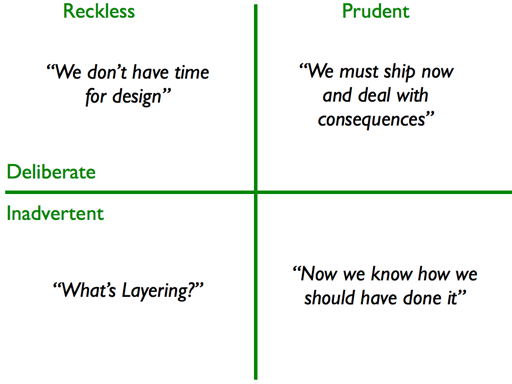
\includegraphics[width=0.5\textwidth]{techDebtQuadrant}
\end{figure}
Martin Fowler, on the other hand, warned against taking on too much deliberate debt. He argues that `Even the best teams will have debt to deal with as a project goes on - even more reason not to overload it with crummy code.'\footcite{fowlerTechnicalDebtQuadrant2009}
He created a quadrant between reckless and prudent and deliberate and inadvertent debt. For Fowler, the difference between reckless and prudent is the way the debt is taken on. Reckless debt happens without an appropriate evaluation of the consequences, risking difficulties in the future. Alternatively, prudent debt is taken on
with the trade-offs in mind and the knowledge of the future costs. Fowler differentiates between deliberate and inadvertent in a similar way to McConnell's differentiation between intentional and unintentional debt.
The various combinations of these four elements in the quadrant results in four different approaches. Reckless and deliberate would mean quick solutions without considering the long-term impact. Reckless and inadvertent results in flawed design or implementation, either carelessly or unknowingly. 
Prudent and deliberate is purposefully taking on debt to gain a short-term advantage with plans of repayment and finally prudent and inadvertent means taking on debt due to lack of knowledge or experience.\footcite{fowlerTechnicalDebtQuadrant2009}\\

In their article `Technical Debt: From Metaphor to Theory and Practice' (2012) Kruchten et al.\ criticize the concept of technical debt to be `somewhat diluted lately' \footcite[18]{kruchtenTechnicalDebtMetaphor2012}, stating that every issue in software development was called some form of debt. 
Therefore they set out to define `a theoretical foundation'\footcite[19]{kruchtenTechnicalDebtMetaphor2012} for technical debt.\\
Kruchten et al.\ state that technical debt has become more than the initial coding shortcuts and rather encompasses all kinds of internal software quality comprises.\footcite[19]{kruchtenTechnicalDebtMetaphor2012}
According to them, this includes architectural debt, `documentation and testing'\footcite[20]{kruchtenTechnicalDebtMetaphor2012} as well as requirements and infrastructure debt.
All these debt types allow engineers to better discuss the trade-offs with stakeholders and to make better decisions.\\
\\TODO: More about Kruchten and Theory?

There have been many studies providing empirical evidence for the theoretical concepts of technical debt. Highly influential studies were undertaken by Potdar and Shihab (2014) as well as by Li et al.\ (2015).\\
In their study Potdar and Shihab analyzed four large open source projects to find self-admitted technical debt as well as the likelihood of debt being removed. They found that `self-admitted technical debt exists in 2.4\% to 31\% of the files.'\footcite[1]{potdarExploratoryStudySelfAdmitted2014}
Additionally, they found that `developers with higher experience tend to introduce most of the self-admitted technical debt and that time pressures and complexity of the code do not correlate with the amount of the self-admitted technical debt.'\footcite[1]{potdarExploratoryStudySelfAdmitted2014}
They also discovered that `only between 26.3\% and 63.5\% of the self-admitted technical debt gets removed'\footcite[1]{potdarExploratoryStudySelfAdmitted2014}. This relatively low removal rate of self-admitted technical debt indicates a wider challenge:
developers recognize the issues of their implementation, but defer remediation potentially leading to a major impact on long-term maintainability.\\
Another approach to provide empirical evidence towards technical debt was taken by Li et al.\ . They conducted a systematic mapping study to `get a comprehensive understanding of the concept of "technical debt"'\footcite[194]{liSystematicMappingStudy2015}, as well as obtaining an overview of the current research in the field.
Areas of investigation included existing types of technical debt (TD), the effect of technical debt on software quality and quality attributes (QAs) as well as the limit of the technical debt metaphor.\\
They established that the `10 types of TD are requirements TD, architectural TD, design TD, code TD, test TD, build TD, documentation TD, infrastructure TD, versioning TD and defect TD.'\footcite[215]{liSystematicMappingStudy2015}
Additionally they found that `[m]ost studies argue that TD negatively affects the maintainability [\ldots] while other QAs and sub-QAs are only mentioned in a handful of studies'\footcite[215]{liSystematicMappingStudy2015}.\\
During their studies,  Li et al. observed that the inconsistent and arbitrary use of the term `debt' among researchers and practitioners can cause confusion and hinder effective management of technical debt.\footcite[211]{liSystematicMappingStudy2015} Additionally practitioners `tend to connect any software quality issue to debt, such as code smells debt, dependency debt and usability debt.'\footcite[212]{liSystematicMappingStudy2015}
This indicates an inflationary use of the term, which is important to keep in mind when speaking about technical debt.\\

The implications these studies have for the software industry are significant. They show that software decay and technical debt are tangible and measurable in real world software projects.
In their paper `Software complexity and maintenance costs' (1993) Banker et al. empirically demonstrated that `software maintenance costs are significantly affected by the levels of existing software complexity.' \footcite[12]{bankerSoftwareComplexityMaintenance1993}
This finding emphasizes the important of proactively managing the software quality and addressing debt early in the project lifecycle, to keep the complexity and therefore cost to a minimum.\\
To address these effects, practitioners strongly recommend refactoring. Fowler argued in his book `Refactoring: Improving the Design of Existing Code' (2019)
that `[w]ithout refactoring, the internal design - the architecture - of software tend to decay.'\footcite[58]{fowlerRefactoringImprovingDesign2019}
To prevent this, he suggests `[r]egular refactoring [to] help[s] keep the code in shape'\footcite[58]{fowlerRefactoringImprovingDesign2019}.\\
To prevent long-term issues, practitioners recommend actively managing technical debt through refactoring, tracking and other strategies 
that integrate debt management into the software development process.\\

\subsubsection{Conclusion}

This chapter has outlined the foundational challenges inherent to software engineering and introduced two critical concepts: software decay and technical debt.
Drawing on Frederick Brooks' distinction between essential and accidental difficulties, it becomes evident that complexity, changeability and lack of uniformity are deeply rooted in the nature of software itself and cannot be fully resolved.
These enduring challenges are the foundation of the concepts of software decay and technical debt.\\

Software Decay refers to the gradual degradation of a software system's internal quality, leading to reduced maintainability, increased complexity and higher change effort. This is a natural outcome of continuous system evolution in a response to changing requirements and environments.
As shown through empirical work of Eick et al. and the theoretical contributions of Lehman and Parnas, software that is not actively maintained becomes harder to main, less modular and more fragile, making decay a systematic and long-term threat to software sustainability.\\

On the other hand, technical debt captures the intentional or unintentional compromises made during software development that create short-term advantages but lead to long-term costs. Originating as a metaphor, it has since evolved into a structured framework for describing, architectural design, code or process-related liabilities.
While software decay can be seen as a developing property of ongoing change, technical debt often originates from conscious decisions. Whether this is due to deadlines, insufficient knowledge or lack of resources, it manifests through debt like code quality deterioration, architectural erosion or insufficient testing.\\

Importantly, technical debt and software decay are closely related: unmanaged technical debt accelerates software decay, while software decay can lead to the accumulation of technical debt. Empirical studies from Potdar, Li and Banker confirm the measurable impact of these phenomenon on maintenance costs, defect rates and overall system quality.\\

To effectively manage these issues, the software industry has developed strategies that go beyond reactive maintenance. Structured, proactive practices such as continuous refactoring, rigorous quality assurance, technical debt management and large scale testing are essential to prevent the accumulation of debt and decay.
Based on these foundations, the next chapter will explore concrete mitigation strategies in commercial environments providing a comprehensive overview of the most common strategies, techniques and frameworks used in the industry to address technical debt and software decay.\\

\subsection{Mitigation Strategies in Commercial Environments}
As discussed in the previous section, technical debt and software decay have been recognized as significant challenges in the software industry. They can lead to 
increased maintenance costs, reduced software quality and decreased developer productivity, overall resulting in a more expensive and less competitive product.
With these challenges in mind, practitioners and researchers have developed a variety of strategies which manage, prevent and mitigate technical debt.
This section will provide an overview of the most common strategies, techniques and frameworks used in commercial environments to address technical debt.
This will be viewed on different levels: high-level strategies, code-level practices, architectural level as well as process and organizational measures.\\

\subsubsection{High-Level Mitigation Strategies}
To efficiently mitigate software decay and technical debt, proactive management strategies are essential. These strategies aim to prevent the accumulation of 
debt and address software entropy and decay directly by integrating quality assurance into everyday development process.
Such strategies include Agile methodologies like Scrum or \ac{XP} as well as technical practices
such as \ac{CI/CD}. These practices are designed to embed ongoing maintenance and quality assurance into routine workflows, thus combating software entropy at its core.\\
Agile methods emphasize frequent iterations, close collaboration between developers and stakeholders as well as continuous refactoring to prevent the
gradual degradation of software quality and mitigation of software decay.\\
Similarly, \ac{CI/CD} introduces rigorous automation, rapid feedback loops and early detection of defects to proactively control both technical debt accumulation
and broader software quality decay. Collectively, these methodologies create a culture of continuous improvement, adaptability and quality assurance, 
ensuring software maintainability and long-term project sustainability.\\

\paragraph{Agile Methodologies}
In their paper `Technical Debt Management in Agile Software Development: A Systematic Mapping Study' (2024)\footcite{leiteTechnicalDebtManagement2024} Leite et al.
investigated how agile methods can be used to manage technical debt. They found that `\ldots Scrum and Extreme Programming are the most utilized methodologies 
for managing technical debt.'\footcite[318]{leiteTechnicalDebtManagement2024} While this study focuses explicitly on technical debt, both Scrum and \ac{XP}
also inherently address the broader issue of software decay by encouraging proactive quality management and continuous improvement practices.\\
Scrum was first presented by Ken Schwaber in his paper `SCRUM Development Process' (1997)\footcite{schwaberSCRUMDevelopmentProcess1997}. 
It has since become one of the most popular agile frameworks in the software industry. Scrum explicitly manages software quality and technical debt through iterative cycles called sprints.
After each sprint, the team reflects on their work, identifies quality issues, technical debt and potential decay indicators and plans improvements in
retrospectives. Leite et al. found that the most used artifacts for identifying technical debt in Scrum are the Sprint and Product Backlog.\footcite[315]{leiteTechnicalDebtManagement2024}
By explicitly managing these items with their workflow, teams effectively reduce both debt and software entropy, improving overall software maintainability.\\

\ac{XP} was first introduced by Kent Beck in his influential book `Extreme Programming Explained' (1999)\footcite{beckExtremeProgrammingExplained1999}.
It explicitly integrates practices to enhance software quality and directly prevent software decay.
\ac{XP} practices such as pair programming, \ac{TDD}, \ac{CI} and continuous refactoring help maintain high software quality, thus preventing both debt accumulation
and broader software entropy.
Pair programming prevents decay by securing higher-quality code through collaborative review and knowledge sharing between developers.
\ac{CI} provides regular, frequent code integration, significantly reducing integration complexity and associated decay risks.
\ac{TDD} establishes robust test coverage, catching defects early and preventing quality erosion.
The effectiveness of refactoring, a cornerstone XP practice, has been proven empirically. For example, in their case study (2008) Moser et al.
demonstrated that refactoring explicitly `prevents an explosion of complexity'\footcite[262]{moserCaseStudyImpact2008}
and promotes simpler, easier-to-maintain designs.
They found it drove developers toward simpler designs, reducing complexity, coupling and long-term maintenance issues thereby directly counteracting software decay.\footcite[262]{moserCaseStudyImpact2008}
Beck argues that \ac{XP}'s incremental, continuous quality practices consistently maintain software quality and adaptability throughout development, directly addressing both debt and broader software decay.\\
On the whole, agile methodologies, particularly Scrum and \ac{XP}, systematically manage technical debt and proactively prevent software decay by fostering continuous improvement, structured quality management and adaptability.
Complementing these Agile practices, the adoption of automated \ac{CI/CD} pipelines further enhances the proactive management of both technical debt
and broader software decay through rigorous quality control and systematic automation.\\

\paragraph{Continuous Integration/Continuous Deployment}
\ac{CI} was first introduced by Beck in the context of \ac{XP} and later refined by Martin Fowler in his influential article `Continuous Integration'\footcite{fowlerContinuousIntegration2006}.
Fowler describes \ac{CI} as not only the frequent, automated integration of code into the main repository but also the systematic automation of building and testing process.
According to Fowler, `Self-testing code is so important to Continuous Integration that it is a necessary prerequisite.'\footcite{fowlerContinuousIntegration2006}.
Furthermore, another critical prerequisite is `that they can correctly build the code,'\footcite{fowlerContinuousIntegration2006} thus guaranteeing that code changes consistently
integrate without issues.\\

To further prevent technical debt and broader software decay by maintaining a specific code quality, quality analysis tools such as static code analyzers like SonarQube or DeepSource are frequently integrated into
\ac{CI} pipelines. These tools often provide a metric to evaluate technical debt which is calculated based on the effort in minutes to fix the found maintainability issues.\footcite{sonarqubeUnderstandingMeasuresMetrics2025}
In their paper `Technical Debt Measurement during Software Development using Sonarqube: Literature Review and a Case Study' (2021)\footcite{murilloTechnicalDebtMeasurement2021}
Murillo et al. found that SonarQube is a useful tool for early debt detection. The estimated remediation effort metric allows for a good debt management prioritization.\footcite[5]{murilloTechnicalDebtMeasurement2021}
However during their research they noticed if they changed SonarQubes default rules by just 26 rules, the technical debt effort would increase from
1 hours and 50 minutes to 11 hours.\footcite[4]{murilloTechnicalDebtMeasurement2021} This issue, together with the fact that SonarQube can only detect code related debt if correctly configured as well as no other debt such as
infrastructure or requirements debt, makes these tools useful but not a complete solution.\\

\ac{CD}, introduced by Jez Humble and David Farley in their foundational book `Continuous Delivery: Reliable Software Releases through Build, Test and Deployment Automation' (2010)
extends \ac{CI} by automating the entire software release pipeline. \ac{CD} ensures that the software is always in a releasable state.
According to Humble and Farley, implementing a functional \ac{CD} pipeline `creates a release process that is repeatable, reliable and predictable'\footcite[17]{humbleContinuousDeliveryReliable2010}.
Beyond predictability, additional significant benefits include team empowerment, deployment flexibility and substantial error reduction.
Specially, \ac{CD} effectively reduces errors, particularly those introduced by poor configuration management, including problematic areas such as
`configuration files, scripts to create databases and their schemas, build scripts, test harnesses, even development environments and operating system configurations'\footcite[19]{humbleContinuousDeliveryReliable2010}.\\

\subsubsection{Code-Level Practices for Preventing Decay}
On the code level, a variety of practices can be used to prevent software decay and technical debt. The two major practices have been previously introduced: continuous refactoring and maintaining software quality.\\
The benefits of refactoring have been demonstrated in the previous section. However, deeper empirical research illustrates the impacts and challenges in a commercial environment.
Kim et al. (2014) observe in their paper `An empirical study of refactoring challenges and benefits at Microsoft' that `[d]evelopers perceive that refactoring involves substantial cost and risks'\footcite[17]{kimEmpiricalStudyRefactoring2014}.
Additionally they describe the benefits refactoring brings as `multidimensional'\footcite[17]{kimEmpiricalStudyRefactoring2014}. Furthermore it is not consistent across different metrics, leading to their recommendation of a tool to monitor the impact of refactoring across these metrics\footcite[17]{kimEmpiricalStudyRefactoring2014}.
Similarly, Tempero et al. (2017) established certain barriers to refactoring in their study `Barriers to refactoring'. They found that at least 40\% of the developers in their study would not refactor classes, even though they thought it would be beneficial. \footcite[60]{temperoBarriersRefactoring2017}\\
Tempero et al. claims the reasons were `lack of resources, of information identifying consequences, of certainty regarding risk and of support from management'\footcite[60]{temperoBarriersRefactoring2017} even though developers did not state a lack of refactoring tools as a reason.
To eliminate these barriers, Tempore et al. suggest refactoring should be goal-oriented instead of operations-oriented and a better quantification of the benefits refactoring should bring to better reach a decision.\footcite[61]{temperoBarriersRefactoring2017}\\
Both studies show that the theoretical benefits of refactoring are not always directly translated into the industry. Developers often perceive refactoring as risky and costly, even though they are aware of the benefits.\\

\ac{TDD} is another code-level practice previously introduced. It was first formally described by Kent Beck in his book
`Test Driven Development: By Example' (2002) in which he argues that writing tests before the implementation
encourages cleaner code and gives developers the confidence to tackle complex problems.\footcite[pp. 8-9]{beckTestdrivenDevelopmentExample2002}
This practice promotes modularity, testability and clean design, key characteristics in preventing software decay. By focusing solely on code
that fulfills predefined tests, developers are guided toward creating small and focused code, which is loosely coupled. These qualities make systems
easier to maintain and refactor, directly counteracting long-term degradation.
Multiple studies have confirmed the quality-enhancing effects of \ac{TDD}.
In an empirical study, Mäkinen and Münch (2014) found that  TDD most commonly led to a reduction in defects and increased maintainability, 
although its effect on overall software quality was more limited.\footcite[13]{inproceedings}
Importantly, they note that TDD significantly improves test coverage, a key factor in preventing unintentional decay.
These gains, however, were accompanied by higher development effort.\footcite[13]{inproceedings}\\
This is consistent with the case study by Bhat and Nagappan (2006), who reported a 15-35\% increase in development time when using \ac{TDD}.\footcite[361]{bhatEvaluatingEfficacyTestdriven2006a}
However they also observed that `the resulting quality was higher than teams that adopted a non-TDD approach by an order of at least two times.'\footcite[361]{bhatEvaluatingEfficacyTestdriven2006a}
Similarly, Bhadauria et al. (2020) confirm TDD’s positive effect on code quality and defect reduction.
Interestingly, their study found that for less experienced developers, TDD did not lead to increased development time and was associated with higher developer satisfaction.\footcite[1058]{bhadauriaPerformanceOutcomesTestDriven2020}\\
These findings indicate that TDD can significantly improve code quality and maintainability two critical factors in preventing software decay.
However, the trade-off in development effort and time must be carefully considered, which may explain TDD's limited adoption in the industry.\\

\subsubsection{Architectural Strategies for Long-Term Quality}
In addition to code-level practices, the maintenance of the software architecture is essential for preventing software decay and architectural-level technical debt. 
Architecture erosion, characterized by increasing divergence from the intended design due to continuous modifications and changing requirements,
significantly impacts maintainability and introduces substantial technical debt.\footcite[1]{desilvaControllingSoftwareArchitecture2012}
One common strategy to mitigate these risks,  is architecture conformance checking, a process ensuring code changes comply with predefined design rules.
De Silva and Balasubramaniam (2012) emphasize that proper documentation, dependency analysis and compliance monitoring are critical prerequisites for
effectively employing this strategy.\footcite[135]{desilvaControllingSoftwareArchitecture2012}\\
Beyond mere conformance, teams must also embrace managed architectural evolution, adapting architectures systematically rather than reactively. Such evolution
should actively balance new requirements with long-term sustainability to avoid uncontrolled erosion.\footcite[34]{liUnderstandingSoftwareArchitecture2022}
A key component in this proactive approach is managing the architectural technical debt. These structural design decisions could impact future adaptability if not
carefully controlled. Besker et al. (2016) suggest a framework to systematically identify, analyze and address architectural debt to preserve structural integrity.\footcite[11]{beskerManagingArchitecturalTechnical2018}\\
Nevertheless, when architectural decay becomes substantial, teams face critical decisions between incremental refactoring and radical redesigns.
Nord et al. (2012) highlight that systematic impact analysis, guided by explicit architectural metrics, is crucial for making informed decisions on when substantial 
redesign becomes necessary to substantially restore software quality.\footcite[99]{nordSearchMetricManaging2012}\\
Practical tooling, such as automated architectural monitoring and recovery solutions, plays a significant supportive role in these efforts. 
The detailed application and empirical evidence of such tools issue discussed thoroughly in the subsequent section on Tool Support for Continuous Quality Assurance.\\

In summary, proactively maintaining software architecture is essential for mitigating long-term software decay. Architecture conformance checking 
prevents the inadvertent erosion by ensuring adherence to established design principles. Managed architectural evolution further ensures that the architecture
can sustainably adapt to changing requirements without introducing uncontrolled structural degradation. Moreover, explicitly recognizing and managing architectural
technical debt enables targeted interventions before significant decays occurs. Ultimately, strategic decisions on refactoring versus comprehensive redesign should be 
guided by systematic architectural analysis, metrics and empirical evaluations to ensure long-term maintainability and quality.

\subsubsection{Process and Organizational Measures}
Organizational and process-oriented practices form the third pillar in combating software decay.
One crucial practice is the management of technical debt. Many companies track technical debt items like outdated modules, quick fixes or known architectural shortcomings.
This can be done through issue trackers or backlogs to allow for structured approach and time allocation to address them regularly.
An industry-wide survey conducted by Ramač et al. (2021) found that 47\% `had some practical experience with TD identification and/or management'\footcite[40]{ramacPrevalenceCommonCauses2021}.
By visualizing and tracking technical debt, teams can prioritize and address debt items systematically, preventing their accumulation and broader software decay.
Ramač et al. also found that the most common cause for technical debt was time pressure caused by deadlines\footcite[40]{ramacPrevalenceCommonCauses2021} and the `single most cited effect of TD is delivery delay.'\footcite[40]{ramacPrevalenceCommonCauses2021}
This indicates that time pressure is not only a cause of technical debt but also a consequence, leading to a vicious cycle of debt accumulation and delivery delays. To break this cycle, a balance of new development and maintenance is crucial to prevent a border software decay.\\

Another important practice is conducting regular code reviews as part of the development workflow. This practice dates back to 1976 when Michael Fagan reviewed the benefits of peer code inspections.\footcite[183]{faganDesignCodeInspections1976}
He found that `inspections increase productivity and improve final program quality.'\footcite[205]{faganDesignCodeInspections1976}
Since then, code reviews have become more lightweight compared to the inspection proposed by Fagan, increasing participation. By removing in-person meetings and reviewer checklists, accelerating and simplifying the process, code reviews have become a standard practice in software development and usually occur before code is merged into the main repository.
McIntosh et al. (2016) investigated the impact of code reviews on software quality by comparing the review coverage, participation and expertise of the reviewer against the post-release defects.\footcite[6]{mcintoshEmpiricalStudyImpact2016}
They found that coverage, while important, is not the only factor that influences the post-release defects.\footcite[39]{mcintoshEmpiricalStudyImpact2016}
They state that `review participation should be considered when making integration decisions.'\footcite[39]{mcintoshEmpiricalStudyImpact2016}
Additionally, they recommend that if an expert in the matter is not available for the original code, they should be included in the review process to prevent defects.\footcite[39]{mcintoshEmpiricalStudyImpact2016}

In conclusion, structured approach to managing technical debt and preventing software decay is crucial to maintain software quality and long-term project sustainability.
Process-integrated practices like code reviews, explicit technical debt control and a culture of continuous refactoring create an environment that proactively manages software decay and technical debt.

\subsubsection{Tool Support for Continuous Quality Assurance}
To further support the proactive management of software decay, technical debt and the overall code health over time, a variety of tools have established themselves in the industry.
Automated quality assurance tools are often integrated into modern development processes. A common approach, as previously mentioned, is the use of \ac{CI} pipelines. These can be used in combination with quality gates which use static code analysis to block additions to the code base that do not meet the quality standards e.g. a 
certain code coverage, complexity or maintainability threshold. This allows developers to catch issues early and rectify them before they are introduced into the code base . While the concept of quality gates is not new, the automation of these gates have recently been investigated by Uzunova et al. (2024).
They found that these gates can serve as a check point to assess software metrics like code coverage, bug density or compliance with coding standards. \footcite[8]{uzunovaQualityGatesSoftware2024}
To allow for this kind of automation, they suggest tools like SonarQube, Sigrid or Maverix.ai. These tools provide real-time feedback allowing for an enforcement of quality criteria.\footcite[8]{uzunovaQualityGatesSoftware2024}\\
Utilizing this approach enables developers to catch issues early and prevent the introduction of technical debt and software decay into the codebase.\\

As discussed in a previous section, ensuring that changes do not divert from the original architecture design is crucial to prevent the erosion of the architecture.
To support this, tools have been developed to automatically detect architecture violations. These tools are able to collect information about the architecture from the source code
and compare it to the proposed architecture.\footcite[6]{thomasStaticDynamicArchitecture2017} In their case study 
`Evaluating an Architecture Conformance Monitoring Solution' (2016), Caracciolo et al. investigated three different tools to detect architecture violations:
SonarQube, Sonargraph and TeamCity\footcite[43]{caraccioloEvaluatingArchitectureConformance2016}. They concluded that their approach 
`can be applied in an industrial context.'\footcite[44]{caraccioloEvaluatingArchitectureConformance2016}
They furthermore argue that the tools can be conveniently added to a dashboard, allowing for a short feedback loop as well as proactive management of architectural violations.\footcite[44]{caraccioloEvaluatingArchitectureConformance2016}
These benefits can be seen in their case study, where they observed that the overall violations decreased from 606 to 600 in an 18 year old system with one million lines of code\footcite[43]{caraccioloEvaluatingArchitectureConformance2016}.
Based on these project parameters Caracciolo et al. `consider that to be a positive outcome.'\footcite[43]{caraccioloEvaluatingArchitectureConformance2016}\\

Numerous empirical studies show the effectiveness of these tools. In their paper `Empirical investigation of the influence of continuous integration bad practices on software quality' (2022),
Silva and Bezerra found that `CI can improve software quality, especially about cohesion.'\footcite[4]{silvaEmpiricalInvestigationInfluence2022} However they also observed the impact
of bad practices in the implementation of CI. They found that the quality levels were incorrectly set and the standard configuration tools were used instead of 
adjusting them to the project needs, which overall harmed the software quality indicators. \footcite[4]{silvaEmpiricalInvestigationInfluence2022}
This indicates that, for the tools to be effective, they need to be correctly configured and adjusted to the project needs.\\

\subsubsection{Synthesis of Commercial Mitigation Strategies}
Effectively managing software decay and technical debt requires a balanced combination of technical, architectural and organizational strategies.
At the highest level, Agile methodologies and \ac{CI/CD} frameworks foster proactive maintenance cultures, reducing entropy through incremental improvement
and automated quality assurance. On the code level, disciplined practices such as continuous refactoring and \ac{TDD} have empirically demonstrated their effectiveness
in maintaining modularity, testability and reducing technical debt - with the downside of a higher development effort. Architectural strategies complement these
by ensuring structural integrity through systematic conformance checks, managed evolution and explicit handling of architectural technical debt, especially as
the scale or requirements of projects evolve.

Organizational measures such as technical debt tracking, dedicated maintenance cycles and structured code reviews provide essential process-level support,
enabling teams to systematically prioritize and address decay risks before they escalate. Finally, the strategic use of modern quality-assurance tools, integrated
into \ac{CI} pipelines and architectural monitoring systems, ensures continuous, automated and actionable feedback, thereby enabling developers to maintain
software quality proactively. Ultimately, integrating these diverse practices into a combined quality culture is vital for sustainable software development,
reduced maintenance costs and the long-term viability of software products.\\


\subsection{Unique Constraints in Military Software Development}
\subsubsection{Introduction to Military Software Context}
Software development for military significantly differs from commercial software due to unique demands for high reliability, rigorous security and extended system lifecycles.
The \ac{NRC} book `Reliability Growth: Enhancing Defense System Reliability' (2015) highlights the differences between commercial and military software development.\\
According to the NRC there are three main distinctions. The first regards the `sheer size and complexity of defense systems'\footcite[31]{nrc2015defense}.
These systems often have a vast amount of individual elements which need to work together, and also evolve over time as the architecture  between the different stages of 
the lifecycle changes.\footcite[32]{nrc2015defense} In addition, the \ac{NRC} highlights the fact that new systems have to interact with legacy systems, which can be a challenge
due to the different technologies and architectures used.\footcite[32]{nrc2015defense}\\
The second distinction is the different perspectives of the actors involved. Unlike in the commercial environment, where it is usually only the project manager 
who controls the vision and the goals of the project, in the military environment there are multiple stakeholders with different goals in mind.\footcite[32]{nrc2015defense}
Although the book specially focuses on the American military, the same can be said for the German military.\\
The third difference given by the NRC are the concerns risk. In the commercial environment, the manufacturer has a self-interest in the product being successful and reliable.
In the military environment, however, the government is the customer and often holds most of the risk, as they will be using the product in the end.
The NRC claims that this means `the system developers do not have a strong incentive to address reliability goals early in the acquisition process'\footcite[33]{nrc2015defense}.
especially because the downstream benefits are not quantifiable for the developers.\footcite[33]{nrc2015defense}\\
In her presentation on `A perspective on military software needs', Heidi Shyu highlights additional challenges in military software development.
She argues that, in addition to the complex setting, there are often a multitude of contractors working together, who must interoperate with each other in real time.\footcite[11]{shyu2017military}
These projects often have a lifecycle of decades compared to the commercial software lifecycle of a few years.\footcite[14]{shyu2017military}
Due to these long lifecycles, the software needs to be developed so it can be easily maintained and updated, while still working with legacy systems
which often have very specific requirements.\footcite[14]{shyu2017military}
Whereas the the architecture has to last for decades, soft- and hardware changes much faster, often resulting in a patchwork of quick fixes.\footcite[15]{shyu2017military}
Heidi Shyu provides examples of necessary software solutions such as a flexible architecture which allows for easy updates and additions, self-testing modular code and intuitive, easy-to-use interfaces.\footcite[17]{shyu2017military}\\

In summary, these challenges in military software development are unique to the industry. The vast size and complexity of defense systems,
their long lifecycles and the multitude of stakeholders involved all serve to create a complex environment that requires specialized strategies to manage software decay and technical debt effectively.

\subsubsection{Regulatory and Procurement Constraints in the Bundeswehr}
The procurement and regulatory environment significantly shapes military software development in the German Armed Forces (Bundeswehr). Unlike in commercial settings,
Bundeswehr software projects are tightly governed by formalized frameworks, rigorous approval processes and comprehensive regulations designed primarily to ensure 
accountability, security and reliability. However, these structures can inadvertently limit agility, prolong software updates and contribute significantly to software decay
and technical debt over time.\\

Bundeswehr software utilizes the `V-Modell XT Bw' as the project lifecycle model. It is a customized variant of the standard V-Modell XT, specifically tailored to Bundeswehr needs and closely integrated with the 
Bundeswehr's overarching procurement framework, \ac{CPM}.
The V-Modell XT Bw is a comprehensive framework that encompasses the planning and execution of software projects in the Bundeswehr.\footcite[6]{bundeswehrVModellXTBw}
It includes detailed guidelines for all parts of the software development process, from roles and requirements engineering to \ac{QA} and product quality.\footcite[pp. 20-21]{bundeswehrVModellXTBw}
However, due to its rigid and sequential nature, the waterfall-based V-Modell XT Bw is known to limit flexibility, making iterative adjustments and agile methodologies not possible.\\

The procurement procedures of the Bundeswehr are outlined by the aforementioned \ac{CPM} which was revised in 2012 after a commission in 2010 found that: 
`Die Streitkräfte erhalten ihre geforderte Ausrüstung zumeist weder im erforderlichen Zeit- noch im geplanten Kostenrahmen.'\footcite[36]{strukturkommissionderbundeswehrBerichtStrukturkommissionBundeswehr2010}.
Due to these problems, the revised \ac{CPM} has an increased focus on upfront requirement definition and comprehensive risk assessments. This creates long lead times
for approval and makes quick technological changes difficult to realize.
In addition, the \ac{EVB-IT}, the standardized contract for government IT solutions, hinders agile development. In his article from 2022,
Holger Schröder claims that multiple different contract blueprints would have to be combined to allow for an agile development project.\footcite{schroederUngeeignetFuerAgile2022}

Collectively, all these requirements and procurement constraints strongly influence software development practices. Control and predictability are prioritized, making
an iterative and agile framework difficult to use. While these procedures promote accountability and reduce risk, they can severely limit a system's ability to evolve over time, thereby fostering conditions under which software decay and technical debt accumulate. 
Adding to this complexity are strong security and compliance requirements, which will be discussed in the following subsection.

\subsubsection{Security and Compliance Requirements}
Military software is obliged to meet stringent security and compliance standards beyond the usual commercial requirements. Due to the sensitive nature of military operations and data,
the software must adhere to both national and NATO standards. These strict requirements result in severe difficulties 
regarding the lifecycle of the product, the software architecture and maintenance practices. The resulting constraints accelerate the accumulation of technical debt and software decay.\\

Like all federal agencies in Germany, the Bundeswehr must adhere to the \ac{BSI} guidelines for IT security, called IT-Grundschutz\footcite{bundesamtfuersicherheitinderinformationstechnikBSIFAQ}. This defines a comprehensive security framework
that includes technical, personnel and infrastructural security measures through the use of several standards. Eventhough these standards Compliance with these standards involves extensive documentation, risk management processes and regular audits. 
This leads to an increase in the complexity and effort required for ongoing software maintenance and updates.\footcite{bundesamtfuersicherheitinderinformationstechnikBSIStandards}\\

In addition to the national regulations, Bundeswehr software systems are obligated to comply with the NATO security standards. These guidelines establish requirements for the handling of classified data, encryption standards and security clearance of personnel.
This is illustrated by the NATO Security Policy (C-M(2002)49) which dictates the handling of NATO-classified information, constraining software flexibility and maintenance practices\footcite[Enclosure B, pp. 1–3; Enclosure F, pp. 1–2]{NATO2002SecurityPolicy}. 
Compliance with NATO standards mandates extensive security accreditation procedures, detailed documentation and comprehensive vetting of software and hardware systems.
These processes slow down software development cycles and restrict flexibility due to the necessity of re-certifying software after significant changes.

Furthermore the Bundeswehr adheres to national classification rules, such as \ac{VS-NFD}. Systems classified under \ac{VS-NFD} require access control, encrypted communications, dedicated network infrastructure and periodic security accreditation.\footcite[see Part 2, pp. 1–3; Part 3, pp. 1–6]{BMI2010VSNFD}
Developers and system administrators need to adhere to strict usage guidelines, which dictate the permissible software, hardware and methods of data handling.\footcite[Part 3, No. 3.1–3.7, pp. 1–5]{BMI2010VSNFD} Compliance significantly restricts the usage of modern technologies such as cloud services or external software libraries, unless explicitly cleared\footcite[Part 3, No. 3.4.1–3.4.5, pp. 4–5]{BMI2010VSNFD}. 
This can be seen in the example of Genua’s secure remote working solution, which complies with both VS-NfD and NATO security requirements while offering functionality typically restricted in classified environments.\footcite{Genua2023VSNFD}

Although essential for operational security, these security and compliance requirements markedly constrain software adaptability and agility. 
Extensive documentation, mandatory security certifications and regular audits mandated by national and international regulations considerably increase the maintenance workload and complexity. 
Consequently, prolonged approval processes and heightened architectural complexity often accelerate software decay and technical debt accumulation, complicating extensive refactoring or proactive architectural evolution.

In summary, security and compliance requirements play a pivotal role in shaping Bundeswehr software development practices, significantly influencing architecture design, 
maintenance methodologies and lifecycle management. While crucial for safeguarding operational security and classified information, these rigorous standards often inhibit software adaptability and innovation, exacerbating the challenges of software decay and technical debt inherent in military software systems.

\subsubsection{Legacy Systems and Extended Lifecycles}
Legacy systems and extended lifecycles impose particularly significant constraints for military software projects, especially within the Bundeswehr. 
Unlike commercial software, which typically operates for a limited period, military systems frequently remain operational for decades due to high investment costs, complexity and risk aversion to adopting new technologies. Such prolonged operational 
lifespans inevitably contribute to technical debt accumulation and progressive software decay, significantly complicating maintenance and increasing lifecycle costs.

A prominent example of these challenges emerged within the Bundeswehr's logistics and support IT systems at the turn of the century. According to Sebastian Stein's 2011 blog entry,
the Bundeswehr managed around 1,200 distinct outsourced IT systems, creating a highly fragmented and inefficient infrastructure.\footcite{steinBusinessProcessManagement2011} To address this issue, the Bundeswehr initiated the \ac{SASPF} program, consolidating procurement, accounting, 
and logistics systems into a single, integrated SAP-based solution. However, standard SAP software met initially only around 70\% of the Bundeswehr's unique operational requirements, necessitating extensive custom development and temporary workarounds.\footcite{steinBusinessProcessManagement2011} These integrations were further 
complicated by stringent regulatory requirements, diverse stakeholder interests and interoperability challenges with outdated technologies. Consequently, significant technical debt and complexity accumulated, extending the modernization effort well over a decade and clearly demonstrating the severe maintenance implications of legacy systems.\footcite{steinBusinessProcessManagement2011}

Another illustrative case within the Bundeswehr is the Luftwaffe's Tornado fighter jet program. Development began in 1981 and the aircraft entered operational service in 1992. Today, approximately 80 Tornado jets remain operational, with plans for 
replacement only by 2030 resulting in a lifecycle of nearly 50 years.\footcite{skibaTornado50Jahre2024} Continuous software updates have been crucial throughout this extensive period, including notable upgrades like the integration of the RecceLite reconnaissance system in 2009.\footnote{bundeswehrTornado} However, 
each update has progressively become more complex and costly due to aging hardware, software architecture limitations and stringent compliance demands. This incremental layering of software modifications directly contributes to accelerated software decay, increasing the difficulty and expense of maintaining operational effectiveness.

Comparable challenges are also prevalent among international NATO allies. A notable example was highlighted by Kynan Carver (2022), describing how the U.S. \ac{DOD} continued operating critical strategic systems reliant on severely outdated technologies, 
including 8-inch floppy disks, until the late 2010s.\footcite{carverTechnicalDebtCybersecurity2022} Carver emphasizes that maintaining these aging software infrastructures consumes significant financial and operational resources, limiting investment in innovation and proactive modernization strategies.\footcite{carverTechnicalDebtCybersecurity2022}

In conclusion, effectively managing technical debt and mitigating software decay within military systems requires strategic, long-term investments, proactive modernization plans and an explicit focus on maintainability. Addressing the unique challenges posed by legacy 
systems and extended lifecycles is thus crucial for sustaining operational capability and flexibility within an increasingly dynamic military technology environment.

\subsubsection{Conclusion}
Military software development is fundamentally shaped by demands that are far beyond those of the commercial environments. The need for extremely reliable, long lasting systems which still meet strict classification regimes and multi-layered stakeholder requirements creates a highly regulated and risk-shy context.
These characteristics collectively contribute to a development landscape where software decay and technical debt are not merely byproducts of poor practices but structural risks embedded within the system's lifecycle.\\

As shown throughout this section, four constraint areas amplify these challenges. Firstly, the inherit complexity of military systems, often designed to operate for decades, creates pressure to extend the viability of aging platforms.
Secondly, the rigid procurement and development frameworks, such as the V-Modell XT Bw and the \ac{CPM} process, prioritize upfront control and traceability over agility, hindering adaptive or incremental development practices.
Thirdly, extensive national and NATO security requirements impose detailed compliance burdens, restricting the use of modern tools and leading to prolonged certification cycles. Finally, the heavy reliance on legacy systems and technologies, as illustrated by the Tornado jet or SASPF, 
reinforces technical inertia and raises the cost and difficulty of modernization efforts.\\

Together, these factors present a software ecosystem where continuous improvement, architectural evolution and proactive quality management are severely constrained. Consequently, technical debt tends to accumulate more rapidly and opportunities to refactor or modernize the system are limited due to
procedural, regulatory and operational constraints.\\

Therefore it is crucial to understand how military software practitioners operate within this setting. The next section of this thesis will examine how experts working on Bundeswehr-related software systems experience and address these limitations in practice.
The main focus will be their strategies in managing software decay, handling long-lived legacy systems and the impact of the regulatory environment on their work.

\subsection{Summary of the Literature Review}
Software development faces inherent challenges that have existed for decades. The previous chapters examined these problems from three key perspectives: the foundational problems of software engineering, the mitigation strategies used in commercial environments and the unique constraints faced in military projects.
This summary will highlight the key insights to establish a foundation regarding software decay and technical debt, thereby laying the groundwork for the empirical investigation in the following chapters.\\

\subsubsection{Problems of Software Engineering}
The complexity of software systems, combined with their extended lifecycle and constant evolution, creates significant challenges. As presented by Brooks (1986), essential difficulties such as complexity, conformity, changeability and invisibility are inherent in software development.
In contrast are the accidental difficulties which stem from the tooling and process problems of the current software development practices.
These foundational matters create the two following common issues.\\

The first is software decay which refers to the gradual deterioration of software quality, due to evolving requirements and the constant need for updates and maintenance. This has been empirically validated by Eick et al and theoretically supported by Lehman, Belady and Parnas.\\
The second issue is Technical Debt, a metaphor introduced by Cunningham. Technical Debt represents the cost of implementation or design shortcuts taken to meet immediate needs, which can lead to long-term maintenance challenges. This concept has been further developed by McConnel, Fowler and Kruchten, highlighting the risks and management needs
associated with both intentional and unintentional technical debt. Together, these two concepts create a complex environment where long-term degradation is inevitable unless proactively managed.\\

\subsubsection{Mitigation Strategies in Commercial Environments}
To combat software decay and manage technical debt, commercial software projects have developed a wide range of strategies. These include high-level practices such as agile methodologies like Scrum, \ac{XP} or CI/CD pipelines which embed quality into the daily workflow.
Such practices are complemented by code level-techniques like continuous refactoring, \ac{TDD} or code reviews which help manage the complexity and ensure maintainability. Architectural strategies like conformance checking and managing architectural technical debt support long-term structural integrity.
This is further supported by organizational practices such as backlog tracking of debt, balancing time pressure and cultivating a quality-focused culture. Finally, the use of modern tooling through automated analysis tools (e.g. SonarQube, TeamCity) allows enforcement of standards and early detection of issues.\\

These approaches aim to proactively manage quality and control the complexity, thereby reducing the long-term cost of maintenance. 

\subsubsection{Constraints in the Military Software Environments}
While the challenges of decay and technical debt are universal, military software projects face the following unique constraints that complicate their management.\\

The project structure in the Bundeswehr is defined by the V-Modell XT Bw and the \ac{CPM} processes, which emphasize documentation, predictability and rigid lifecycle phases, making agile practices difficult to implement.
The procurement contracts like the \ac{EVB-IT} further limit flexibility and iterative development. The security and compliance requirements from the BSI, NATO policies and VS-NfD create additional burdens through mandatory certifications, audits and limitations on tooling or external software.
The extended lifecycles and legacy systems that exist in every military environment create decade long systems that need service and have to remain operational while also adapting to new requirements.\\

These conditions result in higher maintenance burdens and slower update cycles and also reduce the ability to refactor or modernize systems. This creates a software ecosystem where decay and technical debt accumulation are accelerated.\\

\subsubsection{Conclusion}
In conclusion, software decay and technical debt are persistent and measurable risks in all software systems. While commercial environments have developed effective mitigation strategies, their applicability in military projects is limited by structural, regulatory and operational constraints.\\

Understanding these differences is essential for designing effective strategies to manage decay and technical debt in military software projects. The next chapter will explore how professionals in military related software projects deal with these constraints in practice, offering real-world
insights through expert interviews. They will provide a deeper understanding on how decay and debt are managed, despite the rigid frameworks and complex environments.





%TC:ignore - ignoriert die folgnden Wörter beim Wordcount in Overleaf

%-----------------------------------
% Literaturverzeichnis
%-----------------------------------
\newpage

% Die folgende Zeile trägt ALLE Werke aus literatur.bib in das
% Literaturverzeichnis ein, egal ob sie zietiert wurden oder nicht.
% Der Befehl ist also nur zum Test der Skripte sinnvoll und muss bei echten
% Arbeiten entfernt werden.
%\nocite{*}

%\addcontentsline{toc}{section}{Literatur}

% Die folgenden beiden Befehle würden ab dem Literaturverzeichnis wieder eine
% römische Seitennummerierung nutzen.
% Das ist nach dem Leitfaden nicht zu tun. Dort steht nur dass 'sämtliche
% Verzeichnisse VOR dem Textteil' römisch zu nummerieren sind. (vgl. S. 3)
%\pagenumbering{Roman} %Zähler wieder römisch ausgeben
%\setcounter{page}{4}  %Zähler manuell hochsetzen

% Ausgabe des Literaturverzeichnisses

% Keine Trennung der Werke im Literaturverzeichnis nach ihrer Art
% (Online/nicht-Online)
%\begin{RaggedRight}
%\printbibliography
%\end{RaggedRight}

% Alternative Darstellung, die laut Leitfaden genutzt werden sollte.
% Dazu die Zeilen auskommentieren und folgenden code verwenden:

% Literaturverzeichnis getrennt nach Nicht-Online-Werken und Online-Werken
% (Internetquellen).
% Die Option nottype=online nimmt alles, was kein Online-Werk ist.
% Die Option heading=bibintoc sorgt dafür, dass das Literaturverzeichnis im
% Inhaltsverzeichnis steht.
% Es ist übrigens auch möglich mehrere type- bzw. nottype-Optionen anzugeben, um
% noch weitere Arten von Zusammenfassungen eines Literaturverzeichnisse zu
% erzeugen.
% Beispiel: [type=book,type=article]
\printbibliography[nottype=online,heading=bibintoc,title={\langde{Literaturverzeichnis}\langen{Bibliography}}]

% neue Seite für Internetquellen-Verzeichnis
\newpage

% Laut Leitfaden 2018, S. 14, Fussnote 44 stehen die Internetquellen NICHT im
% Inhaltsverzeichnis, sondern gehören zum Literaturverzeichnis.
% Die Option heading=bibintoc würde die Internetquelle als eigenen Eintrag im
% Inhaltsverzeicnis anzeigen.
%\printbibliography[type=online,heading=bibintoc,title={\headingNameInternetSources}]
\printbibliography[type=online,heading=subbibliography,title={\headingNameInternetSources}]

%-----------------------------------
% Apendix / Anhang
%-----------------------------------
\newpage
\section*{\AppendixName} %Überschrift "Anhang", ohne Nummerierung
\addcontentsline{toc}{section}{\AppendixName} %Den Anhang ohne Nummer zum Inhaltsverzeichnis hinzufügen

\begin{appendices}
% Nachfolgende Änderungen erfolgten aufgrund von Issue 163
\makeatletter
\renewcommand\@seccntformat[1]{\csname the#1\endcsname:\quad}
\makeatother
\addtocontents{toc}{\protect\setcounter{tocdepth}{0}} %
	\renewcommand{\thesection}{\AppendixName\ \arabic{section}}
	\renewcommand\thesubsection{\AppendixName\ \arabic{section}.\arabic{subsection}}
	\subsection*{Interviewleitfaden – Bachelorarbeit Softwareverfall}

\subsubsection*{Einstieg und Hintergrund}
\begin{enumerate}
    \item Welche Rolle haben Sie aktuell im Bereich der Softwareentwicklung militärischer Systeme? Seit wann sind Sie in diesem Umfeld tätig und wie sieht Ihre typische Projektarbeit aus?
    \item Mit welchen Arten von Softwaresystemen arbeiten Sie hauptsächlich? (z. B. eingebettete Systeme, einsatzkritische Plattformen, Verwaltungssoftware, Legacy-Systeme)
\end{enumerate}

\subsubsection*{Legacy-Systeme und lange Lebenszyklen}
\begin{enumerate}
    \setcounter{enumi}{2}
    \item Welche Herausforderungen begegnen Ihnen beim Umgang mit Legacy-Systemen oder langlaufenden Projekten?
    \item Kommt es im Projektverlauf regelmäßig zu Problemen, die durch veraltete Strukturen oder historisch gewachsene Systeme entstehen?
    \item Welche Auswirkungen haben lange Lebenszyklen auf Wartbarkeit und Weiterentwicklung?
\end{enumerate}

\subsubsection*{Strategien zur Qualitätssicherung}
\begin{enumerate}
    \setcounter{enumi}{5}
    \item Welche Maßnahmen setzen Sie ein, um Softwareverfall oder technische Schuld zu vermeiden oder zu reduzieren (z. B. Refactoring, Reviews, Automatisierung)? Sehen Sie diese Maßnahmen als sinnvoll?
    \item Gibt es Bedingungen, unter denen technische Schuld bewusst in Kauf genommen wird? Wird bewusste Schuld getrackt?
\end{enumerate}

\subsubsection*{Agile Methodik}
\begin{enumerate}
    \setcounter{enumi}{7}
    \item Verwenden Sie agile Methodiken wie Scrum oder XP? Falls ja, wie wirken sich diese Praktiken auf den Umgang mit technischer Schuld und Softwareverfall aus?
    \item Wenn keine agilen Methodiken verwendet werden, wie werden Refactoring und Schuldenabbau sonst durchgeführt?
\end{enumerate}

\subsubsection*{Architekturmanagement}
\begin{enumerate}
    \setcounter{enumi}{9}
    \item Wie wird die Systemarchitektur geplant, dokumentiert und gepflegt?
    \item Wie wird sichergestellt, dass sich die Umsetzung an der vorgesehenen Architektur orientiert, insbesondere bei älteren Projekten?
    \item Welche Herausforderungen treten bei der Weiterentwicklung von Architekturentscheidungen auf?
\end{enumerate}

\subsubsection*{Automatisierung und CI/CD}
\begin{enumerate}
    \setcounter{enumi}{12}
    \item Setzen Sie CI/CD in Ihren Projekten ein? Wie sehen die Prozesse konkret aus und hilft CI/CD gegen die zuvor genannten Probleme?
    \item Welche Werkzeuge und Metriken verwenden Sie zur Qualitätssicherung im Build- oder Deployprozess? Was sind Ihre Erfahrungen mit diesen Werkzeugen? Gab es bestimmte Stärken oder Schwächen, die sich auf die Codequalität oder Wartbarkeit ausgewirkt haben?
\end{enumerate}

\subsubsection*{Reviews und Tests}
\begin{enumerate}
    \setcounter{enumi}{14}
    \item Wie wird bei Ihnen mit Code Reviews gearbeitet? Wer beteiligt sich, und wie wird der Prozess organisiert?
    \item Welche Rolle spielen Tests? Nutzen Sie automatisierte Verfahren wie Unit-Tests oder Test-Driven Development? Gibt es bestimmte Tests, die Ihrer Meinung nach am besten bei der Vermeidung von technischen Schulden helfen?
\end{enumerate}

\subsubsection*{Besondere Rahmenbedingungen im militärischen Umfeld}
\begin{enumerate}
    \setcounter{enumi}{16}
    \item Welche Anforderungen an Sicherheit, Zuverlässigkeit oder regulatorische Vorgaben wirken sich auf Ihre Arbeit aus?
    \item Inwiefern beeinflussen Beschaffungsprozesse oder lange Freigabeschleifen Ihre Projekte in Bezug auf technische Schulden und Softwareverfall?
\end{enumerate}

\subsubsection*{Abschluss}
\begin{enumerate}
    \setcounter{enumi}{18}
    \item Können Sie ein Beispiel nennen, in dem eine Maßnahme zur Reduktion von technischer Schuld oder zur Vermeidung von Softwareverfall besonders erfolgreich war? Was genau machte diese Maßnahme aus Ihrer Sicht erfolgreich?
    \item Gibt es weitere Erfahrungen oder Empfehlungen, die Sie im Zusammenhang mit Softwareverfall oder technischer Schuld teilen möchten?
\end{enumerate}

\subsection*{Interview 1}

Interviewer: Dann schon mal vielen Dank, dass du das Interview mit mir machst. Mal so ein bisschen zum Einstieg: Was ist deine aktuelle Rolle im Bereich der Softwareentwicklung und wie lange bist du dort schon tätig und was ist so deine typische Projektarbeit, die du machst?\\
Int-1: Ja, also ich bin jetzt insgesamt, die Ausbildung in dem Bereich hier mit reingezählt, 15 Jahre dabei. Während diesen 15 Jahren habe ich hauptsächlich Softwareentwicklung, Integration und Tests gemacht. Jetzt mittlerweile bin ich tatsächlich primär im Bereich Integration und Test unterwegs, mache aber teilweise noch im Bereich Softwareentwicklung, Fehlerbehebung, Softwarelieferung und so weiter.\\ 
Interviewer: Was sind deine Hauptsysteme oder wie sehen die aus, woran du quasi hauptsächlich arbeitest? Also sind das eingebettete Systeme, Verwaltungssoftware oder Altsysteme?\\ 
Int-1: Also überwiegend würde ich sagen, könnte man es glaube ich als Altsysteme bezeichnen, weil die Projekte schon sehr lange laufen. Im Grunde genommen sind das die Führungssysteme, wo dann die einzelnen Softwarekomponenten integriert sind.\\ 
Interviewer: Und wenn du sagst, die laufen schon eine Weile, was für Herausforderungen hattest du im Umgang mit diesen alten Systemen und langlaufenden Projekten bereits gehabt?\\
Int-1: Also überwiegend würde ich sagen, gerade in meinem Bereich Testintegration sind es sehr oft Kompatibilitätsprobleme. Das sehen wir auch jetzt zum Beispiel im Bereich Tests mit irgendwelchen Testtools, die einfach auf neueren Versionen nicht mehr laufen oder wo wir die Lizenzen teilweise schon gar nicht mehr bekommen zu erträglichen Preisen. Und ja, im Prinzip halt wirklich dadurch, dass das Ganze so alt ist und es auch vorgegeben ist, wie das Ganze auszusehen hat, also diese ganze Umgebung ist ja quasi vorgegeben, die wir bekommen haben, passen irgendwelche neuen Modell-Tools, die wir gerne benutzen würden, da halt nicht rein. Da muss man dann gucken, dass man Kompatibilitätsprobleme aus dem Weg kommt.\\ 
Interviewer: Und kommt es im Projektverlauf regelmäßig zu Problemen durch die veralteten Strukturen, die du ja auch ein bisschen genannt hattest und historisch gewachsene Systeme, auch auf dem Code-Level?\\
Int-1: Ja, auf dem Code-Level würde ich sagen auch. Es ist natürlich so, dass auch teilweise ältere C++-Versionen oder sowas benutzen, wo neue Befehle etc. dann gar nicht unterstützt werden. Auch im Bereich Test, ist jetzt nicht direkt Softwareentwicklung, aber wenn wir jetzt über Python nachdenken – ich weiß gar nicht, welche die aktuellste Python-Version ist, wir arbeiten noch mit sehr, sehr alten Versionen –, das heißt auch da Kompatibilitätsprobleme. Es ist immer wieder das gleiche Problem, es ist alles sehr alt und es passt mit den neuen Sachen nicht mehr zusammen.\\
Interviewer: Und was für Auswirkungen hat das dann auf die Wartbarkeit und die Weiterentwicklung von diesem System?\\
Int-1: Ja, Problem ist natürlich gerade, wenn man viele ältere Dinge hat, die vielleicht auch gar nicht mehr so geschult oder gelehrt werden, wenn man jetzt neue Kollegen kriegt oder so, die kennen sich mit diesen alten Sachen halt nicht mehr so gut aus. Das heißt, eine Herausforderung ist natürlich, dass diese Know-how-Träger, die es damals mal gemacht haben, vor Ewigkeiten, dass die vielleicht auch nicht mehr da sind und das schafft natürlich eine Menge Probleme. Das hat auf jeden Fall negative Auswirkungen auf das Ganze.\\
Interviewer: Und was für Maßnahmen nutzt ihr, um den Softwareverfall oder technische Schulden zu vermeiden oder zu reduzieren?\\
Int-1: Ja, also ich muss sagen, lange Zeit, also wie gesagt, seit 15 Jahren bin ich schon da und ich habe das Gefühl, dass es lange Zeit gar nicht gemacht worden ist oder sehr wenig. Es wurde sehr schlecht dokumentiert, es wurden wenige Tests automatisiert und auch nicht regelmäßig durchgeführt. Mittlerweile nutzen wir Tools, die halt automatisch die Testkette durchlaufen lassen, dass man auch regelmäßig mal sieht, ob da irgendwie was kaputt gegangen ist oder nicht. Es gibt Tools für Codechecks und so weiter. Also es wird viel normalisiert in dem Bereich, damit man dann den Verlauf in fünf Jahren oder so immer noch gucken kann, ob es auch funktioniert.\\
Interviewer: Und das merkt man dann auch im Nachhinein, dass das früher nicht gemacht wurde oder ist das mittlerweile relativ gut ausgebügelt?\\
Int-1: Also es kommt drauf an, also je nach Projekt. Es gibt Projekte, wo es noch nicht so gut aufgebügelt worden ist. Es gibt Projekte, wo man das jetzt mittlerweile nachgeholt hat, aber man hat, glaube ich, eine ganze Menge Zeit verloren und man hätte, glaube ich, wenn man im Vorwege schon solche Dinge gemacht hätte oder auch andere Maßnahmen, hätte man sich, eine Menge Aufwand sparen können.\\
Interviewer: Und zum Thema Reviews und Refactoring: Macht ihr das mittlerweile auch verstärkt, und war das früher eher weniger auch der Fall?\\
Int-1: Früher fast gar nicht. Also früher gab es quasi einen, der es gemacht hat und einen, der die offiziellen Tests dafür gemacht hat. Das war es. Also, so ein inoffizielles Review nochmal zwischendurch gab es gar nicht. In gewissen Projekten, aber auch nicht in allen, gibt es jetzt mittlerweile, dass es Reviews, Refactoring auch immer zwischendurch gibt. Also diesen agilen Ansatz. Aber nicht in allen Projekten.\\
Interviewer: Und in der Historie betrachtet, sieht man schon, dass es jetzt einen Vorteil gibt, oder merkst du da keinen Unterschied zwischen, wie es vorher lief und ob jetzt weniger technische Schuld gibt?\\
Int-1: Also ich glaube, es ist ein bisschen schwer zu bewerten, weil wir das noch nicht so lange machen. Meine Vermutung ist aber, dass man es auf jeden Fall merkt. Man muss natürlich auch dazu sagen, dass sowas wie Reviews und Refactoring auch wieder Zeit kosten. Also man investiert quasi ein bisschen mehr, um hinten raus hoffentlich was zu sparen. Aber ich glaube, es ist noch ein bisschen zu früh, um jetzt zu sagen, dass es so ist.\\
Interviewer: Und gibt es Bedingungen, wo ihr technische Schuld in Kauf nehmt und wird das dann explizit getrackt oder wird das einfach weitergetragen, wenn irgendwelche Abkürzungen oder so verwendet werden?\\
Int-1: Also getrackt wird es auf jeden Fall nicht. Das wüsste ich jetzt nicht, dass sich das jemand irgendwie merkt, dass da und da irgendwie was noch zu tun wäre. Es wird auf jeden Fall bewusst in Kauf genommen, das habe ich auch sehr oft erlebt. Gründe dafür sind natürlich sehr unterschiedlich. In der Regel würde ich sagen, Zeitmangel.\\
Interviewer: Benutzt ihr agile Methodiken, sei es Scrum oder andere? Und wenn ja, wie wirken sich diese Praktiken auf technische Schuld und Softwareverfall aus?\\
Int-1: Ja, also agil ist tatsächlich ein neues Thema im Bereich militärisch. Das gab es bisher gar nicht. Wir haben es jetzt, also ich war ja in unterschiedlichen Projektes unterwegs, in einem Projekt haben wir es aktiv gemacht. Ich würde sagen, dass es sich grundsätzlich sehr gut auswirkt, dass es sehr sinnvoll ist, auch wie du auch schon sagtest, was Felix sagte, dass man diese Wissensträger nicht so zentriert hat, sondern dass man das so ein bisschen verteilt. Es ist natürlich trotzdem so, dass es nach wie vor Leute gibt, die das eine besser können und welche das andere etwas besser können. Und man investiert natürlich im Vorwege mehr Zeit dafür. Es wird natürlich im Vorwege teurer, damit man hinten raus halt so ein bisschen diese technische Schuld versucht schon mal ein bisschen abzufedern. Ich glaube komplett lässt es sich trotzdem nicht vermeiden, aber zumindest, dass es besser dadurch werden wird.\\
Interviewer: Kannst du etwas zur Architektur sagen von den Projekten, wie die geplant, dokumentiert und wie die gepflegt wird?\\
Int-1: Also ich kann zumindest sagen, dass es da in unserem Bereich feste Vorgehensmodelle dafür gibt, also auch feste Dokumente etc., die abgeliefert werden müssen. Das ist bei uns nach dem V-Modell XT. Das ist ja ein Vorgehensmodell, das dafür genutzt wird. Und ich weiß, dass wir quasi intern Strukturen haben oder intern Strukturen benutzen, die daran angelehnt sind, weil wir es halt auch machen müssen. Wir sind ja dazu verpflichtet.\\
Interviewer: Und das heißt, es gibt auch einen Prozess, der sichergestellt, dass die Umsetzung der Architektur richtig ist, auch wenn das Projekt schon eine lange Zeit läuft?\\
Int-1: Ja, ich würde sagen, es ist bei älteren Projekten so ein bisschen wahrscheinlich, dass auch hier und da mal was vernachlässigt wurde. Aber grundsätzlich gibt es diese Strukturen und es wird auch versucht, sicherzustellen, dass sie eingehalten werden. Natürlich dann eher durch Qualitätssicherung und der Kunde, der halt sagt, dass er gewisse Dinge haben möchte.\\
Interviewer: Hast du von Herausforderungen mitbekommen, die entstehen, wenn man die Architektur noch weiterentwickeln möchte?\\
Int-1: Ja, auch hier kommt wahrscheinlich das Thema Alter wieder so ein bisschen ins Spiel. Also, dass irgendwelche Architekturen oder Systeme sehr alt sind und deswegen gewisse Entscheidungen vielleicht auch im Vorwege schon limitiert sind, wie man sich treffen kann oder halt auch nicht. Ansonsten war ich da jetzt aber nicht so stark involviert.\\
Interviewer: Vielleicht etwas wo du mehr involviert bist: Benutzt ihr eine Form von CICD in euren Projekten? Und wenn ja, wie genau benutzt ihr das? Wie sehen die Prozesse dabei aus?\\
Int-1: Ja, also mittlerweile benutzen wir es. Das ist auch etwas, was vor einigen Jahren erst dazugekommen ist und ein bisschen angetrieben worden ist. Wir nutzen es für die automatisierten Tests. Für die Dokumentengenerierung und so und nutzen es aktuell noch nicht. Das ist ein bisschen zu komplex, was wir da haben, zumindest aktuell. Aber wir nutzen es quasi, um regelmäßig mal die Testkette durchlaufen zu lassen, um zu gucken, ob alles noch funktioniert. Auch wenn man nichts angefasst hat, sagt die Erfahrung, dass irgendwie immer wieder was schief geht. Und so hat man dann immer viel im Überblick. Weil es das ist, was in der Vergangenheit sehr stark vernachlässig geworden ist, würde ich sagen.\\
Interviewer: Und kannst du sehen, dass das gegen die zuvor genannten Probleme einen Mehrwert bringt?\\
Int-1: Ja, auf jeden Fall. Einfach den Überblick zu haben, auf welchem Stand ist das gerade, auch wenn vielleicht irgendwas nicht funktioniert. Aber noch zu wissen, wie viel nicht funktioniert, ist es schon großer Gewinn. Weil da waren wir in der Vergangenheit sehr oft im Dunklen.\\
Interviewer: Und was für Werkzeuge und Metriken benutzt ihr zur Qualitätssicherung? Sei es beim Build- oder beim Deploy-Prozess?\\
Int-1: Ja, hier wird viel noch auf Manual-Reviews gesetzt. Also zum Beispiel, dass unsere Qualitätssicherung sich das alles nochmal anguckt. Ansonsten viel automatisierte Testskripte. Gerade bei den Unit-Geschichten, also wenn wir auf Komponenten-Ebene gucken, es gibt ja auch System-Tests, da wird noch viel per Hand gemacht. Also es wird viel noch durchgeklickert mit Anleitungen, jetzt klicken wir darauf und dann warten wir und so weiter. Ansonsten, ja, mittlerweile nutzen wir auch ein paar Tools, sowas wie Jira oder so, ich weiß nicht, ob das damit gemeint ist, Qualitätssicherung und mit all diesen Issues und so. Sowas wie Jenkins für die automatisierten Test-Sachen und sowas. Und ja, die Erfahrungen damit sind bisher auch sehr gut, würde ich sagen.\\
Interviewer: Gibt es entweder Stärken oder Schwächen, die man dann gemerkt hat an der Code-Qualität, wenn man solche Werkzeuge benutzt hat, dass sich das irgendwie positiv oder negativ auf die Wartbarkeit ausgewirkt hat?\\
Int-1: Ja, also natürlich gerade, wenn man Jira-Issues aufmacht und die so ein bisschen verfolgt, also irgendwelche Fehler einspielt und dann mit Kommentaren, wie man das behoben hat und welche Fehler und dass das einer nochmal nachtestet und so. Das ist natürlich sehr, sehr hilfreich, also dass man noch mal gucken kann, was wurde eigentlich geändert. Auch Dinge, wo man dann auch sowas sieht, ich merke es jetzt gerade bei mir, dass irgendwelche Dinge behoben worden sind im Quellcode, aber in den Testskripten nicht und dann müssen die Testskripte ein paar Jahre später nachgezogen werden. Das ist wahrscheinlich so das Paradebeispiel für technische Schuld und wenn man dann nicht nachvollziehen kann, was im Quellcode geändert worden ist, außer sich vielleicht angucken, welche Zeit sich geändert hat, aber vielleicht nicht warum und wie das funktioniert, dann ist das schon sehr lästig.\\
Interviewer: Zu Code-Reviews: Wie wird damit bei euch gearbeitet und wie sieht das aus, wer beteiligt sich und wie wird der Prozess organisiert?\\
Int-1: Ja, also gerade bei Code-Reviews gibt es ja im Prinzip zwei Möglichkeiten: Es gibt einmal das Code-Review, dass man sich mit einem anderen Entwickler zusammen hinsetzt, also das wäre jetzt im agilen Umfeld zum Beispiel, dass man sich mit einem anderen Kollegen hinsetzt aus diesem agilen Team, der jetzt vielleicht auch gar nicht viel Entwicklungserfahrung hat, aber zumindest einfach mal drüber guckt. Manchmal kann das auch schon hilfreich sein. Ansonsten gibt es dann noch die automatisierte statische Code-Analyse. Da gibt es ja auch Tools für. Die werden bei uns auch in Jenkins quasi automatisiert gemacht. Da wird dann geguckt, ob diese Code-Richtlinien eingehalten werden. Was im Endeffekt ja auch darauf basiert, dass man den Quellcode qualitätssichern möchte.\\
Interviewer: Und wie war das in der Historie, wurde das benutzt? Oder ist das alles quasi in den letzten paar Jahren implementiert worden?\\
Int-1: Also gerade dieses, ich sag mal, gemeinsam drauf gucken, das gab es früher eher so: „kannst da kurz mal drüber gucken“, aber nicht so formal. Also so wie jetzt, dass es halt wirklich vorgesehen ist und auch abgehackt wird, als eigenes Issue. Automatisiert ist es, meine ich, nie passiert, regelmäßig. Die Tools selber gab es schon. Das wurde dann aber, wenn die Software geliefert worden ist, mal gemacht. Weil es dann halt mitgeliefert werden muss, dieses Zertifikat, dass es gesichert worden ist. Aber ansonsten wurde es nicht zwischendurch mal gemacht, um zu gucken, ob noch alles gut ist. Hätte man vielleicht machen müssen.\\
Interviewer: Und was für eine Rolle spielen Tests? Also du meintest ja schon, dass es die Automatisierung und die Unit-Tests gibt. Aber wie sieht das in den Projekten aus?\\
Int-1: Ja, also ich sagte ja schon, also überwiegend nutzen wir eigentlich automatisierte Testskripte. Und das halte ich auch für sehr sinnvoll, gerade weil man die halt automatisiert über Nacht laufen lassen kann. Und das ist aus meiner Sicht auch ein sehr gutes Mittel, gegen diese technische Schuld so ein bisschen, gerade über lange Sicht. Also ich habe es jetzt gesehen, bei gewissen Projekten war es halt so, da hat man die Testskripte ewig nicht angefasst. Aber hier und da haben wir so kleine Änderungen gemacht, aber dies dürften wir eigentlich nicht. So, wie das immer so ist. Das dürfte eigentlich nichts kaputt machen. Und jetzt habe ich gefühlt wieder ein paar Monate gebraucht, um die alle auf Stand zu kriegen. Und das ist halt genau diese technische Schuld, die wir im Vorweg hätten verhindern können, gerade wenn es dann Quellcode-Änderungen gibt, dann die Test-Skripte einfach nochmal direkt durchzufahren, vielleicht auch direkt anzupassen und das nicht erst ein Jahr später zu machen.\\
Interviewer: Also das heißt, die Test-Skripte werden dann getrennt von dir quasi aktualisiert und der Entwickler macht damit quasi gar nichts direkt. Also er ändert den Code, aber dass die Tests laufen, ist nicht sein Auftrag.\\
Int-1: Ja, so sollte es vielleicht sein, ist es vielleicht auch, aber das ist oft nicht gemacht worden, sagen wir es mal. Also das ist bei uns sehr unterschiedlich, manchmal macht es der Entwickler, es gibt ja durchaus auch Komponenten, wo die Entwickler bei den Tests mitgearbeitet haben, oder manchmal ist es halt auch eine komplett externe Person. In meinem Fall war es immer mal gemixt.\\
Interviewer: Und spürst du die Anforderungen an Sicherheit und Zuverlässigkeit und auch die regulatorischen Vorgaben stark bei deiner Arbeit, sodass sie sich darauf auswirken?\\
Int-1: Ja, teilweise schon. Also es kommt noch ein bisschen darauf an. Ich arbeite ja jetzt eher im Test-Integrationsbereich. Da ist es natürlich so, dass ich viel gegen die Anforderungen arbeite. Das heißt, je besser die Anforderungen sind, desto genauer müssen ja auch die Tests sein. In unserem Umfeld sind sie teilweise nicht so genau, dass die Tests dann vielleicht auch nicht immer ganz so zuverlässig und deterministisch sind, wie sie vielleicht sein sollten. Ich glaube aber, es gibt durchaus Projekte, wo ich jetzt aber nicht ganz so beteiligt war, wo im Bereich der Softwareentwicklung, dadurch, dass Programmiersprachen wie Ada oder sowas genutzt werden, wo man das dann schon sehr stark zu spürt.\\
Interviewer: Hast du eine Idee, wie die Beschaffungsprozesse und die langen Freigabeschleifen, die existieren, sich auf die Projekte auswirken? Zum Thema technische Schuld und Softwareverfahren?\\
Int-1: Was ist genau gemeint mit Beschaffungsprozesse und Freigabeschleifen?\\
Interviewer: Felix meinte zum Beispiel, dass es häufig, wenn man dann irgendwelche Änderungen machen möchte, erstmal wieder zurück zum Kunden gehen muss. Und dass man halt nicht sofort Änderungen einführen kann, die man eigentlich gerne machen würde.\\
Int-1: Ja, das merkt man doch sehr stark bei uns. Dadurch das wir sehr viele formale Geschichten haben. Also dieser ganze formale Abnahmeprozess ist bei uns deutlich komplexer als bei anderen, würde ich sagen. Also gerade auch, was wahrscheinlich mit Freigabeschleifen gemeint ist, da haben wir natürlich ganz andere Standards als wahrscheinlich welche, die nicht militärische Software machen. So ist es dann so, dass die Softwareänderungen manchmal 10 Minuten dauern, aber der Prozess mit Testen und Nachweis und Lieferung und Freigabe dann durchaus mal eine Woche in Anspruch nimmt.\\
Interviewer: Und das heißt, es ist auch häufig so, dass Sachen nach hinten geschoben werden, wenn sie vielleicht nicht so dringend sind, dass man sagt, machen wir uns jetzt nicht den Aufwand, sodass dann halt viel irgendwie einfach liegen bleibt?\\
Int-1: Ja, tatsächlich. Das ist glaube ich auch das Problem, was ich vorhin auch angesprochen hatte, dass dann teilweise Testskripte rumliegen und das muss dann ganz schnell gehen mit der Softwarelieferung und dann machen wir später irgendwann mal die Testskripte. Dann stellt man ein paar Monate später fest, die laufen ja gar nicht und keiner weiß warum. \\
Interviewer: Kannst du ein Beispiel nennen von einer Maßnahme zur Reduktion von technischer Schuld oder zur Vermeidung von Softwareverfall, die für dich sehr erfolgreich war? \\
Int-1: Ja, da würde ich die Automatisierung der Testskripte tatsächlich nennen. Dadurch, dass man sie jetzt nicht mehr per Hand anstoßen muss, die über Nacht laufen können und ich quasi ein komplett gesammeltes Ergebnis über alle Komponenten hinweg sehen kann, ist das schon ein großer Gewinn. Also vorher mussten wir die per Hand starten. Wir mussten die Testlogs extra auswerten und so weiter. Das passiert jetzt alles vollautomatisiert. Zu Zeiten, wo niemand im Büro sein muss, das ist auf jeden Fall ein großer Gewinn. \\
Interviewer: Gibt es weitere Erfahrungen oder Empfehlungen, die du im Zusammenhang mit Softwareverfall oder technischer Schuld gerne teilen möchtest?\\
Int-1: Ja, also aus meiner Erfahrung: Testskripte immer direkt nach der Softwareanpassung mit anpassen. Weil selbst wenn man der Entwickler ist und das selber gemacht hat vor zwei Monaten, auch dann kann es schwierig werden, die Testskripte nochmal anzupassen. Also wenn man im Thema drin ist, dann wirklich alles einmal gerade ziehen. Am besten auch Dokumentation, wenn die irgendwo da ist, den Quellcode dokumentieren. Also Kommentare schreiben ist auch sehr, sehr hilfreich, sehr wichtig. Sowohl in der richtigen Software als auch an den Testskripten. Das darf man auch nicht unterschätzen. Dadurch kann man, glaube ich, eine ganze Menge Softwareverfall und auch gerade technische Schuld irgendwie in den Griff kriegen. Und man tut der nächsten Generation auch einen großen Gefallen, wenn man das einigermaßen lesbar und gut dokumentiert hinterlässt.\\

\subsection*{Interview 2}
Interviewer: Erstmal zum Einstieg generell: Was für eine Rolle hast du im Bereich der Softwareentwicklung von militärischen Systemen inne, seit wann bist du in dem Umfeld tätig und was ist so die typische Projektarbeit für dich?\\
Int-2: Also prinzipiell, ich bin seit über 20 Jahren hier im Bereich tätig. Ich habe dementsprechend auch öfters gewechselt. Derzeit bin ich Product Owner für ein Teilsegment oder ein Teilsystem, das wir pflegen und warten, das eben auch schon seit 20 Jahren in Betrieb ist. Ich habe aber in der Zeit vorher auch als Entwickler, Tester, Qualitätssicherer, Testmanager, also alles Mögliche mal gearbeitet.\\
Interviewer: Und was ist so deine typische Projektarbeit derzeit?\\
Int-2: Es gibt jetzt zwei Projekte, an denen ich hauptsächlich arbeite. Das eine ist eine Softwareänderung, an der wir gerade arbeiten. Also ich bin in beiden Fällen eben Product Owner. Das heißt für mich eben hauptsächlich, die Arbeitspakete sinnvoll zu verteilen und zu schneidern und eben auch mit unseren ARGE-Partnern, also mit der Thales und der Atlas zusammen abzustimmen, wie unsere Anforderungen eben zu interpretieren und umzusetzen sind. Und gleichzeitig versuche ich eben auch als Entwickler und Qualitätssicherer nochmal einen Blick drauf zu werfen, was gemacht wird und in letzter Instanz eben auch zu kontrollieren, dass das vernünftig gemacht wird, was am Ende dann auch geliefert werden soll.\\
Interviewer: Und an was für Arten an Software-Systemen arbeitest du derzeit hauptsächlich? Also eingebettete Systeme, einsatzkritische Systeme oder Verwaltungssoftware oder sowas in die Richtung?\\
Int-2: Wir haben hauptsächlich ein verteiltes System, in dem eben Prozesse auf diversen Konsolen laufen, die sich dann über Producer-Consumer-Listen oder Publisher-Subscriber eben anmelden können, welche Nachrichten sie kriegen und schreiben wollen und dann darüber Informationen austauschen mit anderen Systemen. \\
Interviewer: Du hast ja schon gesagt, dass die Anwendung 20 Jahre alt ist. Was für Herausforderungen begegnen dir dann im Umgang von solchen Altsystemen oder allgemein langlaufenden Projekten?\\
Int-2: Ja, das hat oft damit zu tun, dass Leute das Projekt irgendwann verlassen und neue Leute dazu kommen. Aber auch wenn du selbst Quellcode geschrieben hast, ihn dann zehn Jahre später noch warten und verstehen zu müssen, ist eben eine Herausforderung. Das lehrt einen, zurückhaltend zu sein, was komplexe Softwarestrukturen angeht und möglichst den Code lieber ein bisschen einfacher zu halten, besser zu kommentieren und eben dafür zu sorgen, dass jeder den Code später auch noch pflegen kann. Dazu kommt eben, dass wir viele ältere Technologien auch benutzen müssen, weil es vorgegeben ist durch das Projekt und die meisten Leute, die neu in unsere Umfelder hineinkommen, dass die eben keinerlei Erfahrung mit diesen Technologien haben. Deswegen ist es auch da sinnvoll, die Software so zu schreiben, dass eben auch jemand, der noch keine Erfahrung mit diesen ganzen Systemen hat, da eben trotzdem gut reinkommen kann. Also dementsprechend ist ein hoher Maßstab an die Qualitätssicherung zu setzen, auch an die Code-Inspektion, dass der Code gut gepflegt ist, verständlich ist und dadurch eben auch langfristig am Leben gehalten werden kann.\\
Interviewer: Das war dann auch ein Wandel mit der Zeit oder war das schon immer? \\
Int-2: Nein, das war tatsächlich schon immer so. Also wir haben im Projekt auch feste Codierrichtlinien, wo genau solche Sachen festgeschrieben sind. Also vielleicht nicht in diesem Detailgrad, aber wir haben diese Richtlinien, die eben auch dafür gemacht sind, den Code am Ende wartbar zu halten.\\
Interviewer: Und kam es im Projektverlauf regelmäßig zu Problemen durch die veralteten Strukturen oder historisch gewachsenen Systeme oder läuft das eigentlich relativ glatt?\\
Int-2: Eigentlich läuft es relativ glatt. Wir haben eher hauptsächlich den Wechsel der Mitarbeiter, der immer wieder stark ins Gewicht fällt. Dass natürlich immer wieder Leute in Rente gehen und dementsprechend sich immer wieder neue Leute einarbeiten müssen und dadurch immer wieder so ein Umdenken stattfinden muss. Wir hatten es früher sehr stark, dass wir eine Person hatten, die sich jeweils um ein einziges Segment gekümmert hat und die eben auch die Hauptansprechperson dafür war. Davon versuche ich jetzt eben auch wegzukommen, indem wir das Wissen eben auch mehr verteilen, weil es völlig klar ist, dass nicht alle Leute bis zum Ende ihrer Laufbahn hier immer nur in einem Softwareprojekt arbeiten werden. \\
Interviewer: Und was für Auswirkungen haben lange Lebenszyklen auf Wartbarkeit und Weiterentwicklung deiner Erfahrung nach?\\
Int-2: Prinzipiell ist es, wie schon gesagt, eben sehr wichtig, dass von Anfang an darauf geplant wird, dass die Software eben eine lange Laufbahn hat und dass dementsprechend sich jedes bisschen, was man in bessere Wartbarkeit steckt, langfristig rentiert. Normalerweise ist es ja so, dass Quellcode nach ein paar Jahren eben einfach nicht mehr benutzt wird und neu geschrieben werden kann. Das ist bei uns eben auch durch diverse Rahmenbedingungen eben nicht so weit möglich. Dadurch, dass wir auch sehr komplizierte Prozesse haben, kann die Software nicht einfach geändert werden, sondern wir müssen einen recht komplexen Prozess durchlaufen, bevor Software dann geändert, verbessert werden kann. Dementsprechend ist es auch dadurch eben sehr wichtig, dass wir es schaffen, die Software vernünftig zu schreiben, gleich von Anfang an.\\
Interviewer: Und was für Maßnahmen benutzt ihr, um Softwareverfall und technische Schuld zu vermeiden oder zu reduzieren? Also Refactoring, Reviews, irgendwelche Automatisierungen? \\
Int-2: Alles davon. Also prinzipiell benutzen wir immer das Vier-Augen-Prinzip. Neuerdings, also früher war es noch nicht so, aber das habe ich in den letzten Projekten eingeführt, dass wir nach Scrum arbeiten und dabei dann eben auch eingeführt haben, dass alles nochmal gereviewt wird: jede Zeile Code, jedes Dokument, das geschrieben wird. Auch früher hatten wir die Vorgabe für den Quellcode, der am Ende dann an den Kunden geliefert wird, dass immer eine Code-Inspection gemacht werden musste. Dafür wurden auch regelmäßige Reports angelegt, die auch auf Nachfrage dem Kunden vorzulegen sind. Von daher, da wurde schon sehr viel darauf geachtet, aber das wird jetzt eben noch deutlich stärker gemacht. Und wenn das dann nötig ist, kann es eben auch im Review rauskommen, das wir Codestellen nochmal schreiben, Refactoren durchführen. Dies, wenn eben rauskommt, dass manche Teile so einfach nicht pflegbar sind oder nicht vernünftig laufen könnten. Aus dem dritten Punkt, Review, Refactoring und Automatisierung. Genau, also wir haben eben auch sehr viel Arbeit in die Automatisierung von Tests gesteckt, also bei Build und Testautomatisierung haben wir sehr viel gemacht. Einerseits, um eben sicherzustellen, dass keine Seiteneffekte sich einschleichen in die Software, aber andererseits, weil es eben auch eine Art von Wissenskonservierung ist. Also, dass eben langfristig dadurch sichergestellt werden kann, dass kein Wissen verloren geht, weil eben alles in diese Prozesse schon eingebrannt ist und dass jederzeit dadurch nachgeprüft werden kann, wie diese Prozesse funktionieren und es eben auch von jedem nachvollzogen werden kann. \\
Interviewer: Das heißt, du siehst diese Maßnahmen als sinnvoll?\\
Int-2: Ja, definitiv. \\
Interviewer: Gibt es Momente, wo ihr bewusst technische Schuld in Kauf nehmt? \\
Int-2: Prinzipiell klar, also, was heißt technische Schuld? Also, prinzipiell, jeder Quellcode kann natürlich immer noch weiter verbessert werden. Es ist immer ein Abwägen zwischen, die Software muss fertig werden, aber sie soll eben auch gut sein am Ende, also möglichst fehlerarm und pflegbar, wartbar, all das soll sie eben erfüllen. Aber andererseits haben wir auch die Deadlines zu der die Software fertig sein muss. Und die Kosten würden natürlich auch explodieren, wenn wir noch mehr Refactorn oder noch mehr Arbeit reinstecken, um den Quellcode zu optimieren. Von Daher ist es immer eine Abwägung, und natürlich ist es gerade eher gegen Ende der Laufzeit, dass dann doch mal eher in Kauf genommen wird, wenn Software nicht optimal ist, solange eben keine Fehler drin sind. Das ist natürlich auch eine Abwägung. Es geht ja jetzt nur um technische Schulden, sprich, oder was heißt nur, also es geht eben mehr darum, natürlich könnte man den Quellcode noch verbessern an anderen Stellen, aber solange die Software keine Fehler drin hat, von denen wir wissen, kann sie dann natürlich durch die Teststufen durch und eben auch geliefert werden am Ende. \\
Interviewer: Und wenn die dann die Schulden kaufen, werden die dann getrackt oder sind die dann quasi, wenn das Projekt abgegeben wird, weg? \\
Int-2: Das hängt davon ab, was das jetzt für Schulden sind. Also wenn tatsächlich nach dem Test zum Beispiel noch einzelne Fehler auftreten, werden die getrackt. Wenn es jetzt nur um Code-Verbesserungen geht, haben wir teilweise in Jira-Stories dafür mal angelegt oder jetzt in GitLab die dann auch hinterlegt. Aber im großen Ganzen, ja, weil es eben auch so aufwendig ist, solche Sachen dann später nochmal zu verbessern. Wenn es dann wirklich nur um nicht optimale Implementierung geht, dann wurde es dann meistens doch eher unter den Teppich gekehrt. \\
Interviewer: Du hast es hier gerade angesprochen, dass ihr Scrum verwendet. Und weil das ja erst vor Kurzem implementiert wurde: Merkst du einen Unterschied zwischen den Praktiken zum Thema technische Schuld und Softwareverfall?\\
Int-2: Es ist schwierig, das an Scrum festzumachen, weil generell eben auch ein starker Umbruch hier in den letzten Jahren stattgefunden hat. Also, ich habe Anfang 2000 hier angefangen, und da war es eben noch ein etwas älterer Bereich. Viele der Kollegen waren schon deutlich älter als ich. Die haben das dann über Jahrzehnte gemacht und eben auch fortgeführt. Viele von diesen Leuten, die das eben jahrzehntelang gemacht haben, sind vor fünf, sechs Jahren nach und nach in Rente gegangen, sodass sowieso jetzt ein Umdenken stattgefunden hat. Dadurch haben wir eben auch viel stärker lernen müssen, dass eben nicht eine Person immer das Gleiche machen kann, sondern dass immer neue Leute reinkommen. Wir haben viele junge Studenten dazu bekommen oder Leute, die ihr Studium abgeschlossen haben, die jetzt zu uns gewechselt sind. Allein dadurch ist es immer wieder vorgekommen, dass wir da umgedacht und verbessert haben, unser ganzes Verhalten. Und ich fand, auch da hat Scrum eben sehr stark geholfen, dass neue Mitglieder im Team leichter an Bord geholt werden konnten, weil eben weniger diese Keller-Mentalität gelebt wird – dieses ich nehme ein Software-Paket mit, bastle ein halbes Jahr im Keller und komme dann mit dem fertigen Paket wieder. Indem man sich eben viel mehr untereinander austauscht und dementsprechend eben auch viel mehr mit anderen Leuten redet, können neue Leute besser an Bord geholt werden. Und jeder hat besser die Möglichkeit, überall mal reinzuschnuppern und im besten Fall nach ein paar Monaten eben alles von dem Projekt gelernt hat, was es zu lernen gibt. \\
Interviewer: Aber das heißt, ihr benutzt auch Scrum, um Refactoring und Schuldenabbau quasi effektiv zu managen. Habt ihr dann quasi spezifische Tickets, wo ihr dann Refactoring mit einplant, oder wie sieht das aus?\\
Int-2: Ja, es ist eine Art von Review eingeplant und ein Teil des Reviews kann es natürlich auch sein, dass dann hinterher beschlossen wird: So das war Mist, den Quellcode müssen wir wegschmeißen und neu schreiben. Ist gerade erst passiert bei einer unserer Testprozeduren, also kann immer wieder passieren, wir haben jetzt keine festen Refactoring-Tickets, aber prinzipiell ist es jedem freigestellt, eigene Tickets zu erstellen. Wenn also ein Entwickler jetzt feststellt, dass manche Teile dringend überarbeitet werden müssen, kann er dafür ein Ticket erstellen, aber auch da gibt es wieder das Problem, dass wir eben in den zu liefernden Quellcode nicht einfach ohne Verfahren eingreifen dürfen. \\
Interviewer: Und ein kleiner Sprung zur Architektur. Wie wird die geplant, dokumentiert und gepflegt?\\
Int-2: Genau, zu dem ganzen Block werde ich dir nicht zu viel erzählen können, weil die wurde eben ursprünglich Ende der 90er Jahre entworfen, also sogar noch vor meiner Zeit. Und die ist mit den ARGE-Partnern, also unseren Arbeitskollegen aus den anderen Firmen, zusammen abgestimmt. Und an dieser Architektur orientieren wir uns nach wie vor. Das heißt, es werden immer mal neue Prozesse eingeführt oder einzelne Blöcke ausgetauscht, aber die Architektur ist seitdem unverändert und kann eben auch nicht ohne weiteres verändert werden. Wir haben Diagramme, die dafür gepflegt werden, in denen diese Architektur festgehalten ist und nach denen leben wir. \\
Interviewer: Und gibt es einen Prozess, der sichergestellt, dass die Umsetzungen sich an der Architektur orientieren?\\
Int-2: Diese Prozesse sind eher technischer Natur. Wir haben Schnittstellen zu den ARGE-Partnern. Das bedeutet, wir müssen genau definieren wie unsere Prozesse funktionieren, was sie verschicken oder eben verarbeiten. Und dementsprechend ist es für uns sowieso schon schwierig, die Architektur jetzt grundlegend zu verändern, weil wir das alles immer mit den ARGE-Partnern abstimmen müssten. Es gibt immer einzelne Softwarepakete, die auf die Firmen verteilt sind und diese Pakete werden dann von dieser jeweiligen Firma verarbeitet und die Schnittstellen nach außen sind eben fest. Die können nicht ohne weiteres geändert werden. \\
Interviewer: Und weißt du von irgendwelchen Herausforderungen, die bei der Weiterentwicklung von der Architektur aufgetreten sind? \\
Int-2: Nö, da wüsste ich nichts zu. \\
Interviewer: Und jetzt zum Thema Automatisierung, die du ja auch schon angesprochen hattest. Benutzt ihr eine Form von CICD? Und wenn ja, wie sehen die Prozesse dabei aus? Und hilft CICD merklich gegen die zuvor genannten Probleme? \\
Int-2: Also wir benutzen GitLab neuerdings. Hatten vorher Jenkins benutzt, sind jetzt aber auf GitLab umgestiegen. Vorweggenommen, also ich finde, das hilft enorm, dadurch, dass viele Prozesse, die vorher sonst per Hand gemacht werden mussten, immer sehr viel Expertise erfordert haben, oder dann doch mal ausgelassen wurden, wenn die Zeit knapp war. Und so ist man quasi gezwungen, das einmal umzusetzen, zu implementieren, diese ganze CICD-Geschichte. Und von daher, wir haben jetzt Pipelines, die bei jeder Änderung durchlaufen oder auch über Nacht angeschmissen werden, sodass wir jederzeit erkennen können, wenn Sachen eben nicht mehr funktionieren, die vorher alle per Hand gemacht werden mussten. Also vor zehn Jahren war es eben noch so, dass viele von diesen Testprozessen zum Beispiel eben per Hand durchgeklickt werden mussten, was dann zwei bis drei Tage pro Prozess dauern konnte. Was jetzt eben alles vollautomatisch innerhalb von, ich sage mal, der Längstläufer, den wir haben, ich will nicht zu sehr ins Detail gehen, aber es funktioniert eben automatisch im Hintergrund. Von daher muss man selber da keine Arbeit mehr reinstecken. Und vor allem, man kann es nicht auslassen. Also es wird ja automatisch gemacht, sodass man automatisch einen auf die Finger bekommt, wenn sich da irgendwelche Sachen eingeschlichen haben. \\
Interviewer: Und das ist jetzt eine Veränderung, die in den letzten paar Jahren kam?\\
Int-2: Also Jenkins haben wir schon länger am Laufen, aber wir haben es eben nach und nach immer weitergetrieben. Also wir haben die CICD-Pipeline immer mehr erweitert. Ursprünglich war es eben eine Build Pipeline, wir haben aber viel Zeit in die Testautomatisierung gesteckt. Wir haben noch andere Tools mit in die Pipeline aufgenommen, die auch die Codequalität prüfen. Die Build Pipeline wird eben auch ausgewertet, ob durch den Compiler irgendwelche Warnings ausgeworfen werden und sowas. Von daher, die Pipeline wächst immer weiter und dadurch wird immer weiter automatisiert und das Arbeiten wird immer praktischer und bequemer auch für die Kollegen. \\
Interviewer: Du hast es ja gerade schon angesprochen und vielleicht musst du nicht alles erwähnen, aber was für Werkzeuge und Metriken verwendet ihr für die Qualitätssicherung? Und was sind deine Erfahrungen mit diesen Werkzeugen bezüglich der Codequalität?\\
Int-2: Genau, wir benutzen Logiscope, nennt sich das Tool. Das ist ein Tool, das eigene Metriken hinterlegt hat, das aber auch erweitert werden kann um neue Metriken. Und die Grenzwerte für diese Metriken, die sind innerhalb der ARGE festgelegt worden, zusammen mit dem ÖAG, also mit unserem Auftraggeber. Und diese Richtlinien sind eben auch einem Prozess unterworfen, durch den die definiert werden. Das ist teilweise eben auch Teil der Schwierigkeit, diese Metriken genau festzulegen, ich weiß nicht, inwiefern du auf Metriken und sowas eingehst in deiner Arbeit. Das Problem ist eben, dass ja immer Grenzwerte geprüft werden, ob diese verletzt werden oder nicht. Also zum Beispiel, ob eine Methode zu komplex ist vom Aufbau. Also zu kompliziert, unverständlich dadurch am Ende. Das wird ja auch anhand von festen Parametern geprüft. Und diese Parameter können eben festgelegt werden. Die sind noch ein bisschen im Wandel, weil wir da eben selbst noch in der Findungsphase sind, was da vernünftige Werte sind, weil sich teilweise die Metriken eben auch widersprechen. Also das ist eben auch ein bisschen so, man muss Erfahrung mit reinbringen aus den Projekten, was dann jetzt am Ende vernünftige Werte dafür sind. Aber trotzdem ist es eben wichtig, dass am Ende dann nochmal jemand drauf guckt, weil es immer Verstöße gegen Metriken geben wird und die dann am Ende bewertet, ob sie an diesen Stellen dann gerechtfertigt sind oder ob sie ausgearbeitet werden sollten. Aber trotzdem finde ich, es ist enorm hilfreich, dass man auf diese Metriken erstmal hingewiesen wird, automatisiert durch die Software. Im besten Fall arbeiten wir eben auch daran, das auch in die Pipeline hineinzubringen, damit die Pipeline das dann eben auch direkt macht, aber dass dann eben auch so ein aktives Nachdenken darüber stattfindet. Als Entwickler neigt man doch eher dazu, den schnellen Weg zu nehmen, einfach eine Prozedur runterzuschreiben, wie man sich das vorstellt und wenn dann hinterher eine Metrik dann nochmal sagt, oh, die ist aber nicht gut strukturiert, ist das sehr hilfreich, wenn man das eben schon beim Schreiben dieser Prozedur berücksichtigt. \\
Interviewer: Habt ihr bemerkt, dass sich dieses Achten auf die Qualität und Wartbarkeit ausgewirkt hat?\\
Int-2: Definitiv. Also kurz zum Beispiel, viele Methoden sind eben kürzer geworden, leichter lesbar und sowas. Das es eben auch einem Laien dann leichter fällt, der neu ins Projekt reinkommt, zu verstehen, was da jeweils passiert. \\
Interviewer: Du hattest ja schon angesprochen, dass ihr jetzt sehr stark auf Code Reviews achtet. Wer beteiligt sich und wie wird das Ganze organisiert?\\
Int-2: Prinzipiell, da wir GitLab benutzen, funktionieren viele Teile dieser Code Reviews einfach online. Da können sich die Entwickler nun selber darunter absprechen. Also wie gesagt, jede Änderung wird eben nochmal gereviewt. Und das hängt so ein bisschen davon ab, was für eine Art von Review da notwendig ist. Also gerade bei unseren Test-Skripten sind wir natürlich relativ frei. Die verlassen unser Haus nicht. Da ist unser eigener Anspruch das einzig Entscheidende. Und eben, dass unsere Qualitätssicherungen am Ende sagt, unsere Tests sind ausreichend gewesen. Ein etwas höherer Maßstab muss eben bei Software angelegt werden, die wir an den Kunden liefern, die am Ende dann auch in Betrieb gehen sollen. Und da sind noch ein bisschen höhere Maßstäbe dran, wie das dokumentiert wird. Und am Ende dann eben auch nachvollziehbar gezeigt werden kann, dass solche Reviews stattgefunden haben, was die Ergebnisse waren. Das wird jetzt alles auch in GitLab dokumentiert, sodass es auch Jahre später dann noch nachvollzogen werden kann.\\
Interviewer: Zum Thema Tests hattest du schon gesagt, dass ihr auch auf Automatisierung umgestiegen seid. Haben bisher diese Tests auch geholfen, technische Schulden zu vermeiden und Softwareverhältnisse zu verhindern? \\
Int-2: Das ist schwierig, weil wir die automatisierten Tests eben nach und nach eingeführt haben. Und wie gesagt, es ist eben schwierig, im Nachhinein die Software zu ändern, wenn wir keinen Auftrag haben, dafür genau diesen Quellcode anzupassen. Deswegen sind wir etwas eingeschränkt mit den Möglichkeiten. Trotzdem haben wir die Möglichkeit eben genutzt, wenn Software sowieso geändert werden sollte, dann haben wir da eben auch Verbesserungen eingeführt. Trotzdem waren unsere Tests auch vorher schon sehr gut, muss ich sagen. Es ist hauptsächlich der Komfort, der dadurch gestiegen ist und dadurch eben auch die Möglichkeit, die Tests regelmäßiger und öfter durchzuführen. Das Problem war selten, dass die Software nicht gut funktioniert hat, sondern meistens, dass die Tests dann eher nicht oft genug durchgefahren wurden und deswegen noch Probleme in den Tests vielleicht drin waren. Und die Qualität unserer Tests ist jetzt einfach deutlich gestiegen und sie werden einfach viel öfter durchgefahren, wodurch einfach viel früher auftaucht, wenn Probleme in der Software enthalten sind. \\
Interviewer: Haben die Anforderungen an Sicherheit, Zuverlässigkeit und auch regulatorische Vorgaben einen Einfluss auf eure Arbeit?\\
Int-2: Sehr großen Einfluss, je nachdem, was für Software wir da gerade pflegen. Es gibt verschiedene Einstufungen. Je kritischer die Software, desto höher ist eben auch der Einfluss, den es auf unsere Arbeit hat, weil desto höher ist eben auch der Testaufwand, den wir zum Beispiel dann betreiben müssen oder desto höher sind die Ansprüche an die Software, die dann die Software auch befriedigen muss. \\
Interviewer: Wie beeinflussen die Beschaffungsprozesse und die Freigabeschleifen das Projekt in Bezug auf technische Schulden und Softwareverfall?\\
Int-2: Wären die Prozesse einfacher, wäre die Software wahrscheinlich besser. So ist es doch oft das Problem, wie du schon meintest vorher, dass wir irgendwelche Fehler feststellen, oder nicht Fehler, Fehler ist noch eine andere Sache, aber das wir Sachen in der Software feststellen wie toten Code, wo man normalerweise sagen würde: ok, schmeißen wir raus. Code, der nicht erreicht werden kann, sollte rausgeschmissen werden. Weil die Prozesse ebenso aufwendig sind, wird das dann eben normalerweise nicht gemacht. \\
Interviewer: Also kommt das auch von der Kundenseite her, dass das quasi ignoriert werden sollte, oder kommt das von eurer Seite, dass man sagt, das ist es nicht wert? \\
Int-2: Beides so ein bisschen. Also die Prozesse sind ja mit den Kunden abgestimmt oder sind auf Wunsch des Kunden. Und die Prozesse haben auch durchaus ihren Sinn. Weil unsere Software so kritisch ist, ist es eben durchaus richtig, dass nicht jeder einfach so in der Software irgendwie rumfuscht und dann vielleicht nicht gut genug getestete Software am Ende produktiv geht. Von daher ist es sehr, sehr wichtig, dass wir diese Prozesse haben, aber andererseits führt es natürlich genau zu diesem besprochenen Problem. \\
Interviewer: Hast du ein Beispiel, in dem eine Maßnahme zur Reduktion von technischer Schuld oder Verbreitung von Softwareverfall besonders erfolgreich war, deiner Meinung nach? \\
Int-2: Also wir hatten jetzt gerade eben, hatte ich vorhin schon angesprochen, einen Testfall, der eben nicht gut war, also schlecht zu lesen. Aber der damalige Kollege arbeitet hier nicht mehr. Von daher musste jemand Neues diesen Quellcode eben pflegen, wo wir genau in das Problem reinlaufen von schlecht wartbarem Code. Es kommt immer wieder vor, dass andere Leute den Quellcode pflegen müssen als die, die ihn vorher geschrieben haben. Und da haben wir, nachdem sich der Kollege da zwei Wochen mit dem Quellcode beschäftigt hat, beschlossen, wir schmeißen ihn weg und schreiben ihn komplett neu. Weil in diesem, also es war ein Test-Skript, von daher kein echter Quellcode, der geliefert wurde. Von daher haben wir eben auch die Freiheit einfach zu sagen, wir werfen ihn weg und machen ihn neu. Dadurch ist er jetzt viel besser, viel wartbarer, viel lesbarer geworden, viel kompakter und hat am Ende auch keinen Fehler mehr geworfen. \\
Interviewer: Und gibt es noch weitere Erfahrungen oder Empfehlungen, die du im Zusammenhang mit Softwareverfall und technischer Schuld teilen möchtest? \\
Int-2: Außer nochmal eben die Aussage, Wartbarkeit ist eben sehr, sehr wichtig, langfristig, mehr wüsste ich jetzt nicht. \\

\subsection*{Interview 3}

Interviewer: Zum Einstieg: Was ist denn eine aktuelle Rolle im Bereich der Softwareentwicklung und wie lange bist du in dem Umfeld tätig? \\
Int-3: Ja, also ich mache jetzt für eine Komponente der F124, die jetzt gerade weiterentwickelt wird, an ein paar Stellen kleinere Änderungen. Da mache ich die Automatisierung in Pipeline, in GitLab, gucke, dass die Oberflächentests automatisiert durchlaufen in einen Container. Dafür habe ich den Container gebaut und dafür gesorgt, dass die Automatisierung da vorangeht, damit wir immer einen getesteten Zustand haben, weil wir in der Vergangenheit auch oft gemerkt haben, wenn man Test lange nicht macht, laufen sie dann irgendwann nicht mehr und man wusste nicht warum. In Zukunft sollen sich bei jedem Commit, muss also alles getestet werden und nächtlich auch jede Komponente. Daran arbeite ich und ja, nebenbei noch eine Automatisierung der Dokumentation. Das ist mein Schwerpunkt aktuell.\\
Interviewer: Und wenn du von diesen Systemen redest, welcher Art sind die hauptsächlich? Sind das eingebettete Systeme oder irgendwelche Legacy-Systeme oder Verwaltungssoftware?\\
Int-3: Ja, also die Software, die da eingesetzt wird, die ist teilweise schon, ich glaube, von 1999 oder so, also die ist schon länger im Einsatz. Ich würde es nicht als Embedded-Systeme betrachten, aber es sind halt wie so, ja, geht schon so ein bisschen Richtung Microservices, wo man halt kleine Prozesse hat, die über eine Infrastruktur, eine Kommunikationsinfrastruktur mit anderen Prozessen kommunizieren können, indem sie Pakete schreiben, Pakete empfangen und das halt teilweise auf Oberflächen darstellen können. \\
Interviewer: Und welche Herausforderungen hattest du bisher, wenn du mit Legacysystemen und langlaufenden Projekten umgegangen bist?\\
Int-3: Also für mich die größte Herausforderung ist, dass man die Sachen nicht einfach starten kann auf seinem Rechner. Wir haben halt eine Entwicklungs-VM gehabt, und man musste dann immer auf einer anderen VM entwickeln, wenn man mal was testen will, den Source-Code auf die HDI, also auf die VM zum Testen und zum Bauen packen. Dort wurde die Software erst gebaut und dort konnten dann die Tests durchlaufen werden. Das ist halt schon ein langwieriger Prozess, wo dann auch schnell mal irgendwie bei Copy-Paste irgendwas falsch kopiert werden kann. Und ja, das macht es grundsätzlich schwieriger, loszulegen, weil da sehr viele Dinge ineinandergreifen, die man berücksichtigen muss, um einen einzelnen Test zu machen. \\
Interviewer: Kommt es im Projektverlauf regelmäßig zu Problemen, die durch veraltete Strukturen oder historisch gewachsene Systeme entstehen?\\
Int-3: Ja, das es gab schon. Also, was ich häufig erlebe, ist, dass es tote Dateien gibt, die über die Historie gewachsen sind, dass irgendwelche Skripte in abgewandelter Form vielleicht vorliegen, die gar nicht mehr verwendet werden und wenn man sich dann initial reinfuchst, um das zu automatisieren, dann kann es halt schnell passieren, dass man mal in einem falschen Skript unterwegs ist. Aber auch ansonsten, in verwendeten Skripten haben wir oft eine Redundanz, die ich bemerkt habe. Das heißt, wenn man dann irgendwie eine Optimierung an einer Stelle macht, muss man sie auch an anderer Stelle machen und ja, das macht das ein bisschen herausfordernd. \\
Interviewer: Und was haben die langen Lebenszyklen für eine Auswirkung auf die Wartbarkeit und Weiterentwicklung, die du beurteilen kannst?\\
Int-3: Ja, also das größte Problem, denke ich, ist vielleicht, dass Leute vor 25 Jahren oder 20 Jahren etwas gemacht haben, die vielleicht gar nicht mehr da sind. Man kann die nicht fragen. Es wurden zwar Dinge in der Erinnerungshistorie festgehalten, aber es kann sein, dass das nicht vollständig gepflegt ist. Das macht es zum einen schwierig, und zum anderen wurden vielleicht über die lange Laufzeit Dinge ausprobiert und nachher nicht wieder richtig entfernt. Also ein simples Beispiel ist, da hat man vielleicht mal hier in der Oberfläche was zeigen wollen, während sie im Test durchlief, hat dann Sleep von 1000 Sekunden eingebaut und vergessen den rauszunehmen. Ja, so was kann halt passieren. Ja, aber grundsätzlich auch durch die Historie, hätte man früher von Anfang an gewusst, wie es am Ende eingesetzt wird, hätte man vielleicht versucht, Redundanzen mehr zu vermeiden. Man hat teilweise auch bei den Tests zum Beispiel viele Dinge doppelt gemacht für einzelne Tests, wo man es hätte vielleicht zentralisiert rauskapseln können, was jetzt zum Teil auch passiert, wo wir aktuell auch viel tun. \\
Interviewer: Das greift schon ein bisschen in den nächsten Punkt, was für Maßnahmen setzt ihr derzeit ein, um Softwareverfall oder technische Schuld zu vermeiden? Also zum Beispiel Refactoring, Code Reviews, Automatisierung, was du ja angesprochen hattest.\\
Int-3: Ja, im Endeffekt all das: Also wir sind jetzt von SVN auf Git umgezogen und wir nutzen jetzt GitLab. Und in GitLab haben wir zum einen halt deutlich schönere Möglichkeiten auch agil zu arbeiten. Wir haben dann quasi ein Backlog, wo wir Issues pflegen, woraus wir die Merge-Requests erzeugen, woraus wir die Branches automatisiert erzeugen, sodass halt auch ein Issue mit dem Merge-Request und mit dem Branch gekoppelt ist. Wenn dann mal was abgeschlossen ist in sich in dem Merge-Request, dann wird das halt auch gereviewt mit mindestens vier Augen, meistens sogar mehr und dann wird das Feedback noch eingearbeitet und das wird alles schön in GitLab festgehalten. Das ist, denke ich, ein Aspekt, der wichtig ist aktuell. Und der zweite Aspekt ist natürlich die Automatisierung, die einfach dafür sorgt, weil früher war so ein bisschen das Problem, die Entwicklung, der Source-Code lag in SVN. Es gab Tests in Jenkins, die wurden zwar automatisch durchgelaufen, aber da gab halt auch Tests, die liefen in Jenkins nicht durch, dann ist man dazu übergegangen zu sagen, die skippen wir jetzt erstmal, weil in der VM laufen sie ja und so hat die Relevanz von diesen automatisierten Tests, ja, hat es an Relevanz gefehlt und sie wurden eher stiefmütterlich behandelt, sage ich mal. Und das wandelt sich jetzt ein bisschen, wir sind jetzt von Testdurchläufen auf einer VM zu Container übergegangen, dass wir auch ganz viele Tests parallel durchlaufen lassen können, so dass man schnelle Ergebnisse bekommt, dass es in GitLab integriert ist und jeder, der ein Issue bearbeitet, auch sicherstellen muss, dass die Tests auch in der Pipeline in den Containern durchlaufen. Und ich denke, das ist ein wichtiger Schritt. Und ja, ein anderer Punkt ist auch, dass wir die Entwicklung vereinfachen wollen, indem wir mehr Container nutzen. Wir wollen die VM da an der Stelle jetzt auch nicht zwingend komplett ablösen, aber es soll halt auch mal schneller möglich sein, in einer Entwicklungs-VM Code zu entwickeln und direkt testen zu können. Dafür sind solche Container halt ziemlich praktisch. Dann starte ich den Container, gucke, baut mein Code, laufen die Tests da drin durch und dann kann ich so guten Gewissens wieder ins GitLab reinpushen. Und ja, das sind alles so Maßnahmen. Und auch ein weiterer Aspekt, der glaube ich nicht zu vernachlässigen ist: Wir haben halt viel auch in Word dokumentiert und für Entwickler ist es, glaube ich, auch einfacher in der Entwicklungsumgebung heraus, da mal schnell was zu dokumentieren und da ist Markdown zum Beispiel auch deutlich angenehmer. Und da wollen wir halt auch die Hürde möglichst runterbringen, damit Leute, wenn sie was ändern, weniger Hürden haben, das auch festzuhalten. Und ja, das ist so ein bisschen das Ziel. Die Hürden möglichst tief runterschrauben, die Qualität möglichst hoch und ja, Refactoring gehört natürlich auch dazu. Also immer, wenn wir jetzt neue Dinge überarbeiten, gucken wir, können wir das an anderen Stellen auch vereinfachen, können wir Sachen zentralisieren. Auch im Rahmen vom Git-Umzug haben wir viel Ballast abgeworfen, was wir jetzt erstmal nicht brauchen. Und das haben wir da auch genutzt. \\
Interviewer: Und was ist das jetzt für ein Zeitrahmen? Also seit wann wird das quasi gemacht? \\
Int-3: Also ich habe angefangen Ende letzten Jahres im November, allerdings mit einem anderen Projekt, aber mit dem gleichen Thema, halt die Containerisierung dieser Entwicklungs-VM. Und ja, das hat relativ schnell geklappt. Und dann bin ich irgendwann Anfang dieses Jahres dazu übergegangen, das halt live in die bestehende Entwicklung einzubringen. Und jetzt wird er halt auch aktiv mit den Pipelines entwickelt. Im Endeffekt seit Anfang des Jahres sind wir da relativ aktiv dabei. \\
Interviewer: Also ist es quasi ein sehr neues Projekt. \\
Int-3: Genau, also die Änderungen, die wir jetzt machen, die sind also relativ frisch. Also wir sind jetzt eigentlich im dritten Sprint, glaube ich, und haben noch zwei vor uns.\\
Interviewer: Und das wirkt ja quasi eher gegen technische Schuld. Aber siehst du irgendwo, dass, wenn technische Schuld irgendwann aufgenommen wurde, ob das je getrackt wurde, wenn es bewusst war, oder ist das quasi eher, ja, wird es aufgenommen und dann passiert es einfach.\\
Int-3: In diesem Projekt versuchen wir natürlich es schnellstmöglich zu beheben, wo es möglich ist. Wir haben tatsächlich Dinge festgestellt, die vertraglich so erledigt wurden, wo sich im Nachhinein gezeigt hat, das war jetzt vielleicht nicht die beste Umsetzung. Auch jetzt, durch das agile Vorgehen mit Scrum im Gespräch mit Kunden. Und dann haben wir halt das auch schnell korrigiert und verbessert. In alten Projekten war es meistens so, dass man Dinge, die man vielleicht besser hätte machen können oder vielleicht besser machen kann. Da haben wir die potenziellen Verbesserungen als Issue aufgenommen und mit einem „Wont do“-Label markiert und dann weggeschoben. So dass wir im Nachgang jederzeit gucken können, das sind Dinge, die wir besser machen könnten. Machen wir jetzt aber nicht, aber sie sind halt festgehalten für die Zukunft, falls wir da nochmal was machen wollen. So versuchen wir, das hier auch zu leben. Aber aktuell gibt es da einfach zu wenig, was wir aufschieben oder wo wir technische Schulden aufbauen. \\
Interviewer: Und bei den anderen Projekten wurde das dann irgendwann angegangen, wenn das auf Wont Do gestellt wurde, oder war das eher zeitlich nie wirklich gewollt?\\
Int-3: Nee, wir haben da halt den Auftrag, wir hatten halt ein festes Budget, wir haben die Sachen auch dokumentiert, den Kunden mitgeteilt, aber da hat sich jetzt keine Folgeauftrag ergeben. Deswegen liegen sie da jetzt erstmal. Aber wenn da was kommen sollte, könnten wir sie wieder rausholen und daran arbeiten. \\
Interviewer: Und du hast ja gerade angesprochen, dass ihr agile Methodiken verwendet. Und merkt man, dass sich diese Praktiken auf Umgang mit technischer Schuld und Softwareverfall auswirken?\\
Int-3: Ich denke schon. Dadurch, dass wir täglich miteinander reden und täglich Fragen stellen und im Review mit anderen Personen zusammensitzen, da wird sowas dann halt immer, glaube ich, gefördert, dass man solche Dinge festhält und mitnimmt. Also wir hatten tatsächlich auch schon Issues, wo wir gesagt haben, das geht jetzt ein bisschen über das hinaus, was wir geschätzt haben für das Issue. Der Scope ist zu groß geworden, und wir haben das dann abgekapselt in ein eigenes Item und dann noch den nächsten Sprint geschoben. Und so versuchen wir halt, die Dinge mitzunehmen und ich glaube, da hilft das agile Vorgehen tatsächlich. Weil wir dann halt auch in einem Sprint-Review gucken, was hat gut geklappt und beim Planning nochmal gucken, was wollen wir jetzt machen. Und ja, Dinge, die dann halt hohe Prio bekommen, die können wir auch schnell angehen und nicht liegen lassen. Ich glaube, das würde bei so einem Wasserfallvorgehen schwieriger sein. \\
Interviewer: Und hast du das irgendwie mal mitbekommen, wie das abläuft, wenn es kein agiles Vorgehen gibt, wie dann mit Schuldenabbau oder Refactoring umgegangen wird? \\
Int-3: Ja, wenn ich den Scope jetzt ein bisschen ändere, also ich glaube, intern bei uns nicht, aber es gibt halt in der Beziehung zu anderen ARGE-Partner. Es gibt halt Themen, die fallen uns auf, aber dann gibt es das Projekt nicht her, sowas im Nachgang mal einfach so zu bessern. Weil das Problem ist, alles, was schon ausgeliefert ist, musste schon durch bestimmte Tests durch, durch bestimmte Verfahren durch, hat einen Stempel bekommen. Es ist halt schwierig da noch was nachzubessern. Und dieses starre Vorgehen ist etwas schwierig. Auch wenn es dann nachher um den kaufmännischen Part geht, da kann man dann dem Kunden solche Dinge anbieten. Man kann es transparent machen, aber das sind dann meistens die Dinge, die als erstes wegverhandelt werden. Und das ist halt das Problem, wenn man es über ein Gesamtprojekt sieht. Intern sind wir natürlich immer jederzeit bereit, wenn das halt auch finanziert wird, alles möglichst schnell zu fixen. Aber diese Strukturen darüber hinaus, die machen es halt immer so schwierig. \\
Interviewer: Das heißt dann quasi, technische Schulden oder sowas, wenn sie nicht von uns behoben werden und dann quasi abgegeben wurden, dann bleiben sie eher bestehen über die lange Laufzeit. Es sei denn, sie bilden große Probleme, die wirklich angegangen werden müssen.\\
Int-3: Ja, der Bedarf beim Kunden muss einfach so groß sein, dass er bereit ist, explizit das anzugehen. Aber oft ist das dann für den Kunden einfach attraktiver, ein neues Feature zu nehmen, statt irgendwas Bestehendes nochmal zu korrigieren. Und ja, da ist es dann eine finanzielle Sache. \\
Interviewer: Vielleicht ist es nicht in deinem Projekt direkt sichtbar, aber vielleicht im Generellen. Wie wird die Architektur geplant, wie wird die Architektur dokumentiert, gepflegt in so einem langlaufenden Projekt? \\
Int-3: Ja, also in dem Projekt ist es aktuell halt schwierig, weil wir ja ein kleines Zahnrad im ganzen Konstrukt sind. Da wird vieles halt einfach vorgegeben. Aber in kleineren Projekten, wo ich jetzt auch unterwegs war in dem Kontext, und wenn wir es halt selber machen mussten, die Konzepte gebaut haben, dann haben wir das natürlich alles mit Skizzen dokumentiert und das dann halt auch kommuniziert und besprochen und Verbesserungsvorschläge aufgezeigt. Und ja, das haben wir in dem kleinen Kontext tatsächlich mit Markdown dokumentiert. Und ja, die Bilder mit so einem Editor erstellt und als PDF ausgeliefert. \\
Interviewer: Aber dann in den großen Projekten arbeitet man damit nicht wirklich, sondern nimmt das quasi als Vorlage und jemand anderes kümmert sich dann um Erweiterungen und sowas.\\
Int-3: Also meistens gibt es ja schon eine vorgegebene Kommunikationsinfrastruktur mit festgelegten Schnittstellen, was ja auch gut und wichtig ist. Und dann, wenn wir zum Beispiel einen Prozess bekommen, den wir überarbeiten oder neu erstellen wollen, dann müssen wir uns halt einfach an die Schnittstellen halten. Da kriegen wir von der Architektur selbst wenig mit. Also in einem kleineren Projekt, das wir gemacht haben, da ging es halt auch um eine neue Kommunikationsinfrastruktur. Da haben wir für unseren kleinen Bereich die Konzepte gemacht, haben dann auf Schwachstellen hingewiesen und da können wir jetzt nur darauf hoffen, dass die das in deren Gesamtarchitektur nachher berücksichtigen oder vielleicht an irgendwelchen Stellen schrauben können.\\
Interviewer: Aber wie wird sichergestellt, dass die Umsetzung sich an der vorgelegten Architektur orientiert, auch wenn es ältere Projekte sind? \\
Int-3: Ja, im Endeffekt gibt es ja diese Kommunikationsinfrastruktur, und wenn wir nach dem Standard halt kommunizieren, dann halten wir uns ja indirekt an die Architektur, die gegeben ist. Da können wir halt auch wenig machen. Und da wird das Datenmodell auch vorgegeben. Es kann sein, dass sich da was ändert. Da müssen wir das bei uns gegebenenfalls anpassen und wenn vielleicht irgendwas nicht richtig ist, können wir es halt zurückkommunizieren. Aber da tut sich eigentlich nicht viel.\\
Interviewer: Vielleicht etwas mehr in deine Richtung: Du erwähntest ja schon Automatisierung. Zu welchem Level benutzt ihr dann CICD in euren Projekten, und wie sieht der Prozess genau aus. Hilft dir die CICD bei diesen zuvor genannten Problemen? \\
Int-3: Ja, also ich hoffe, dass es hilft. Das ist ja auch meine Aufgabe. Es ist halt eher auch so, dass wir eine gewisse Qualität nachweisen müssen. Und da gibt es halt verschiedene Parameter, die dann ja gemessen werden, teilweise wie Code-Coverage oder dass man statische Code-Analysen macht. Und es gibt da halt Vorgaben, an die wir uns halten müssen. Und sowas lässt sich halt gut darin abbilden. Und man kann dann durch die CICD, also dann halt eine Pipeline, und wenn an einem Prozess sich was ändert, dann wird der geänderte Prozess quasi in den Container geschmissen. Es wird geguckt, ob immer noch erfolgreich gebaut wird, wenn nicht, was sind die Fehler, dann gibt es ein Report. Wenn das erfolgt ist, dann gibt es die Tests, die dann durchlaufen werden. Und wenn da irgendwas nicht passt, dann gibt es auch da einen Report, dann kann ich in GitLab einsehen, was fehlgeschlagen ist. Ich kriege teilweise Screenshots, wenn ich ein Fehlerbild habe. Und so kann ich dann halt auch so Messwerte wie Test-Coverage mir ausgeben lassen, um halt jederzeit nachweisen zu können, dass sie gut ist oder vielleicht zu niedrig ist und kann da halt gegebenenfalls nachbessern. Und ich glaube halt, der große Mehrwert ist einfach, dass das einfach zu jeder Zeit passiert. Und auch gerade in der agile Softwareentwicklung ist ja der Grundgedanke, dass man am Sprintende ein lieferfähiges Produkt hat. Und wenn du das immer alles händisch testen musst, dann kriegst du das einfach nicht hin. Dann ist man ja zu 90\% der Zeit einfach nur mit Tests beschäftigt, und deswegen hilft uns das da an der Stelle enorm.\\
Interviewer: Du hattest das schon angesprochen. Was für Werkzeuge und Metriken verwendet ihr für die Qualitätssicherung?\\
Int-3: Im Endeffekt ist es so: Wir haben die Testreports, die Units-Reports, die quasi die Ergebnisse der Unittests wiedergeben. Wir haben die Codecoverage als Kennzahl und wir haben die statische Codeanalyse, die uns dann Findings quasi hochwirft, wenn wir hier und dort am Code etwas besser machen können. Und darauf können wir dann reagieren. Und ansonsten muss ich überlegen, was wären Kennzahlen? Noch mehr Kennzahlen? Ich glaube erst mal nicht. Also wir haben grundsätzlich, gerade im Ada-Part, die Möglichkeit, alle möglichen Kennzahlen noch zu messen. Und zwar wie tief zum Beispiel Schleifen gehen können, zu welcher Tiefe, wie viele Verzweigungen etwas nehmen kann. Und über solche Kennzahlen kann man dann halt auch gucken, dass man den Code vielleicht dahingehend optimiert, um ihn einfacher zu halten und wartbarer zu machen.\\
Interviewer: Und habt ihr irgendwelche Stärken oder Schwächen in diesem Bereich herausgefunden, wenn es um Codequalität und Wartbarkeit geht. \\
Int-3: Jetzt im Bezug auf die Automatisierung oder auf den Code selbst? \\
Interviewer: Auf die Automatisierung. \\
Int-3: Ja, also die Stärke habe ich ja gerade so ein bisschen genannt. Im Endeffekt dieses jederzeit lieferfähig sein, jederzeit funktionierenden oder kompilierbaren Code zu haben. Und einen getesteten Code haben, den man theoretisch ausliefern kann. Ich denke, das ist eine große Stärke. Wenn man jetzt eine Schwäche nennen müsste, ist natürlich der Aufwand dahinter, das Ganze so weit zu automatisieren. Aber gerade bei Langlaufprojekten, da rentiert sich das ja sehr schnell. Also wenn das jetzt so ein einmaliges Ding wäre, dann würde man diesen Aufwand vielleicht nicht in der Form betreiben. Aber wir wollen die Software über Jahrzehnte noch pflegen. Das lohnt sich. \\
Interviewer: Also wäre das quasi deine Empfehlung bei neuen Projekten, die voraussichtlich eine lange Laufzeit haben, dass man immer so eine Infrastruktur aufbaut, die so eine Automatisierung erlaubt?\\
Int-3: Also ich denke, grundsätzlich ist es immer, wenn man sich einen Moment aussuchen kann, in dem man diese ganzen Werkzeuge einführt, dann ist es am schönsten, wenn man es direkt zu Beginn macht. Dann profitiert man halt während der Entwicklung am meisten und hat halt auch den geringeren Aufwand als nachher erst eins zu bringen. Das sollte man das am Anfang machen. Und dann muss man natürlich halt immer gucken. Man muss ja auch nicht direkt die ganze Palette machen. Man kann ja mit kleinen Sachen anfangen und dann halt bei Bedarf immer weiter aufstocken. Und halt gucken, was für den Umfang oder für die Pflegbarkeit notwendig ist mit einem Augenmaß. \\
Interviewer: Benutzt ihr eigentlich eine Art von Quality-Gate oder sowas? Oder achtet ihr quasi einfach nur auf die Reports, die dann daraus kommen? \\
Int-3: Also wir machen halt die Code-Reviews. Die werden ja auch festgehalten und auch in den Code-Reviews wird dann immer jede Anmerkung notiert und festgehalten. Und ja, das ist im Endeffekt unsere Qualitätssicherung an der Stelle, wenn es darum geht, eine Lieferung fertig zu machen und mehr halt zum Thema Dokumentation und Vollständigkeit, aber nicht jetzt code-spezifisch, ob das fachlich alles richtig ist. Dann haben wir natürlich auch einen Qualitätssicherer, der da immer nochmal guckt, dass halt die Anforderungen, die wir auch vom Kunden haben, erfüllt sind und dass alles, was im Rahmen dieses ISO-Standards erforderlich ist, auch abgedeckt ist. Also jemanden, der uns halt auf die Prozesse hinweist, haben wir da an der Stelle. Aber es ist halt eher organisatorischer Natur. Dass die entsprechende Dokumentation da ist und so weiter und der Rahmen eingehalten ist. Inhaltlich haben wir halt die Code Reviews. \\
Interviewer: Ja, okay. Aber nichts quasi in der Pipeline selber drin, dass ein Standard eingehalten werden muss, sonst failed die Pipeline oder sowas in die Richtung, sondern man guckt dann einfach quasi auf den Report. \\
Int-3: Also die Pipeline wird rot, wenn ein Test fehlschlägt. \\
Interviewer: Ja gut, aber wenn man jetzt zum Beispiel auf die Metriken, auf die Code Qualität oder auf die statische Analyse oder sowas guckt?\\
Int-3: Ja, nee, da haben wir jetzt aktuell, dass die Metriken ausgegeben werden. Also nur bei den Unit Tests, wie gesagt. Wenn die Tests nicht alle durchlaufen, dann wäre sie rot. Und das ist jetzt für uns ein Zustand, der muss behoben sein, bevor es gemerged wird. \\
Interviewer: Du hast ja schon die Code Reviews angesprochen. Wie laufen die ab? Wer beteiligt sich daran? Und wie wird das generell organisiert? Also du meintest ja, mindestens eine andere Person. Aber wie sieht das genau aus? \\
Int-3: Ja, also bei uns ist es so, dass ein Sprint-Team sagt, eine Person, ich bin jetzt mit meinem Item durch, es wäre Ready zum Review. Und dann meldet sich jemand und dann wird zum Review eingeladen. Und wenn Leute Lust haben, können rein theoretisch auch alle daran teilnehmen, je nachdem wie Zeit ist. Und ja, dann wird das halt mit mindestens vier Augen gereviewt. Aber es wird halt auch ein bisschen darauf geachtet, dass die weiteren zwei Augen auch ja, die Kompetenz besitzen, um das beurteilen zu können. \\
Interviewer: Und das hattest du ja auch schon sehr stark angesprochen. Aber hast du deiner Erfahrung nach den Eindruck, dass die Tests gut gegen technische Schulden helfen? Oder ist es quasi nur eine Absicherung, dass der Code so funktioniert, wie er soll?\\
Int-3: Ja, das ist halt so eine indirekte Hilfe. Die technischen Schulden, die lassen sich in Reviews leichter identifizieren und darauf aufmerksam machen. Aber das Tolle ist ja, wenn sie behoben sind, hast du die Tests, die dann sagen, die Tests laufen immer noch durch. Und es kann natürlich passieren, dass man auch technische Schulden durch die Tests aufdeckt. Also es gab zum Beispiel den Fall, dass nach einem Test nicht alles richtig abgeräumt wurde und beim zweiten Test der Test beeinflusst wurde. Und das ist dann mit dem lokalen Test nicht aufgefallen aber mit den automatisierten Tests schon. Und solche Fehler lasen sich auch dadurch gut auffinden. Und gerade auch wenn Prozesse dazwischenkommen, die dann vielleicht irgendwas nicht richtig abräumen. Ja, aber genauso richtige, bewusste technische Schulden, die werden dann eher auf persönlicher Ebene diskutiert. \\
Interviewer: Kannst du beurteilen, ob die Anforderungen an Sicherheit, Zuverlässigkeit oder regulatorische Vorgaben sich auf die Arbeit von dir auswirken?\\
Int-3: Also nicht aktuell, aber es gibt andere Projekte, da sind natürlich die Anforderungen zum Beispiel an die Code Coverage sehr hoch. Um so eine hohe Coverage zu erreichen von, ich weiß nicht, teilweise sind irgendwie 95\% im Raum, die sind halt natürlich schwierig zu erreichen und das hätte natürlich Einflüsse. Ansonsten versuchen wir auch intrinsisch die Qualität so hoch wie möglich zu halten, auch zum Selbstzweck, damit wir auch selbst ein gutes Gewissen haben bei den Sachen, die wir ausliefern. Von daher würde ich sagen, sind wir eher auch intrinsisch getrieben. Und die Regulatorien sind oft tendenziell eher ein bisschen lascher. Ja, wobei, eine Sache ist zum Beispiel, wenn wir eine Vorgabe bekommen, dass wir mit bestimmten Tools testen müssen, dann ist das natürlich wieder mit extra Aufwand verbunden. Das wäre vielleicht doch dann etwas, was Auswirkungen hat.\\
Interviewer: Inwiefern beeinflussen die Beschaffungsprozesse oder lange Freigabeschleifen die Projekte in Bezug auf technische Schulden oder Softwareverfall?\\
Int-3: Da wären wir wieder bei dem Thema was wir zu Beginn ein bisschen hatten. Wir können zwar technische Schulden oder Fehler melden und kommunizieren. Aber wir sind natürlich darauf angewiesen, dass das auch beschafft wird, dass das behoben wird. Und ohne dass wir einen Auftrag bekommen, dürfen wir halt auch nichts machen. Wir können nicht einfach an Codebestandteilen irgendwas ändern, nur weil wir etwas schöner oder besser machen und korrigieren wollen. So toll es auch ist, wir dürfen es nicht, weil sie sind halt abgenommene Bestandteile. Daher dürfen wir nicht einfach beliebig an irgendwelche Sachen ändern. Darum sind wir in diesem Beschaffungsprozess natürlich gebunden. Und ja, der ist dann heute mal sehr langwierig. Und leider kann man auch nicht ausschließen, dass manche Fehler nie behoben werden. Und das ist halt ein Problem. Deswegen machen wir auch viel Werbung für agiles Vorgehen, wo sowas halt leichter unterzubringen ist.\\
Interviewer: Auf das gesamte Projekt das agile Vorgehen zu verwenden ist eher unwahrscheinlich derzeit? Gibt es da eine Bewegung, die quasi daran interessiert wäre?\\
Int-3: Ja, wir hatten zu den Sprint-Reviews ja auch schon das Beschaffungsamt hier und die sind grundsätzlich schon interessiert und sie sehen auch die Vorteile, aber es ist natürlich auch mit Nachteilen für das Beschaffungsamt dahingehend verbunden, dass sie natürlich mehr Präsenz zeigen müssen, mehr Aufwand unter Umständen haben, das enger begleiten müssen. Was natürlich der Qualität zugutekommt und ich glaube, das Interesse ist da, es tut sich ein bisschen was. Aus meiner Sicht müsste auch nicht alles direkt komplett agil passieren, wenn man halt in den Verträgen schon leichte Spielräume schaffen würde, mal Dinge zu streichen, neue Dinge reinzunehmen, die vielleicht im Laufe des Projekts einfach in der Priorität so eine hohe Gewichtung bekommen, wäre dem Problem schon viel geholfen. Und das ist halt das größte Problem, dass es diese Spielräume aktuell zu wenig gibt oder sie zu wenig genutzt werden.\\
Interviewer: Kannst du ein Beispiel nennen, in dem eine Maßnahme zur Reduktion von technischer Schuld oder zur Vermeidung von Softwareverfall besonders erfolgreich war? \\
Int-3: Eine Maßnahme, wo sie besonders erfolgreich war, also da wir jetzt das, woran ich arbeite, noch nicht ausgeliefert haben? Ja, wenn man das agile Vorgehen an sich nimmt und diese leichte Testbarkeit unsererseits, dann haben wir zumindest einmal schon sehr schnell auf einen Kundenwunsch reagiert und Dinge, die halt sonst einfach vielleicht nicht genutzt worden wären, weil sie zu umständlich umgesetzt wurden, korrigiert und mit wenig Aufwand jetzt umgesetzt haben. Das denke ich jetzt für das agile Vorgehen auf jeden Fall ein Gewinn und hat den Endkunden gezeigt, dass es möglich ist. Und ich glaube halt, es war vielleicht in dem Sinne weniger eine technische Schuld, sondern eine Usability-Schuld, die wir da beglichen haben. Wenn man diesen Mechanismus auch für andere technische Schulden noch umsetzen könnte, wäre es gut. \\
Interviewer: Und was macht die Agilität aus deiner Sicht besonders erfolgreich beim Vermeiden von technischer Schuld?\\
Int-3: Ja, das sind halt diese Spielräume, Dinge anzugehen. Also man hat zum einen eine engere Kommunikation mit dem Endkunden oder Endnutzer und man kriegt halt viel besser mit, was will er eigentlich wirklich. Oft entstehen ja auch Dinge, die er gar nicht so wollte, die aber in den Anforderungen so drin standen und das sind halt so Themen, bei denen finde ich es schwierig, zwischen technischen Schulden und vielleicht organisatorischen Schulden oder irgendwelchen Schulden zu unterscheiden. Es sind halt Dinge, die machen das System komplex, sie führen in die falsche Richtung, verschlechtern die Wartbarkeit und die Nutzbarkeit. Da müssen wir halt mehr ran und ich finde, mit agilem Vorgehen lässt sich das besser machen, halt durch die bessere Kommunikation, durch dieses Sprint-Vorgehen, wo man halt zum Beginn eines Sprints Dinge ganz nach oben nehmen kann, weil sie gerade wichtig sind und ja, das macht es einfacher. Beim Wasserfall kriegt man halt eine Eingabe von ganz vielen Anforderungen, setzt sie nach eigenem Wissen und Gewissen durch, bei manchen Dingen waren die Anforderungen vielleicht schlecht, bei manchen hat man es vielleicht nicht richtig interpretiert, so entsteht halt ein Riesenwust an falschen Umsetzungen und da wäre vielleicht das Thema technische Schulden drin. Wenn dann auf dem letzten Meter noch Dinge schnell hingebogen werden sollen, dann ist das natürlich ein Riesenpotenzial für solche technischen Schulden, dass man da schnell mal was einbaut, nur um irgendjemanden zu befriedigen. Sowas passiert bei einem agilen Vorgehen aus meiner Sicht ein bisschen weniger.\\
Interviewer: Gibt es weitere Erfahrungen oder Empfehlungen, die du in Zusammenhang mit Softwareverfall oder technischen Schulden gerne teilen möchtest?\\
Int-3: Es gab natürlich schon ein Projekt, an dem du auch mitgearbeitet hast, wo man quasi ein Projekt übernommen hat, wo schon etwas ziemlich unsauber war, wo aber aus Zeitgründen auf dieser technischen Schuld aufgebaut hat. Und dann hat man irgendwann eine ganze Stadt draufgebaut und dann kriegt man sie nichtmehr so leicht weg. Grundsätzlich ist der Wille da, es zu beheben, aber das Geld nicht. Und das ist natürlich immer so ein wichtiger Aspekt. Wenn man eigentlich es schöner machen will, aber die Zeit oder das Geld es nicht hergebeben, dann wachsen solche technischen Schulden. Automatisierung schenkt einem Zeit, wenn sie erstmal da ist. Dann kann man sich vielleicht Zeit für sowas nehmen und deswegen bin ich ein großer Verfechter der Automatisierung und auch vom agilen Vorgehen, um technische Schulden nicht zu groß werden zu lassen. \\




\subsection*{Usage of AI}

These interviews were transcribed through a locally run version of OpenAI's Whisper with the model large-v3-turbo.

\end{appendices}
\addtocontents{toc}{\protect\setcounter{tocdepth}{2}}

\newpage
\pagenumbering{gobble} % Keine Seitenzahlen mehr

%-----------------------------------
% Eigenständigkeitserklärung
%-----------------------------------
\section*{%
	\langde{Eigenständigkeitserklärung}
	\langen{Declaration of authorship}}
\langde{Hiermit versichere ich, dass ich die angemeldete Prüfungsleistung in allen Teilen eigenständig ohne Hilfe von Dritten anfertigen und keine anderen als die in der Prüfungsleistung angegebenen Quellen und zugelassenen Hilfsmittel verwenden werde. Sämtliche wörtlichen und sinngemäßen Übernahmen inklusive KI-generierter Inhalte werde ich kenntlich machen.

Diese Prüfungsleistung hat zum Zeitpunkt der Abgabe weder in gleicher noch in ähnlicher Form, auch nicht auszugsweise, bereits einer Prüfungsbehörde zur Prüfung vorgelegen; hiervon ausgenommen sind Prüfungsleistungen, für die in der Modulbeschreibung ausdrücklich andere Regelungen festgelegt sind.

Mir ist bekannt, dass die Zuwiderhandlung gegen den Inhalt dieser Erklärung einen Täuschungsversuch darstellt, der das Nichtbestehen der Prüfung zur Folge hat und daneben strafrechtlich gem. § 156 StGB verfolgt werden kann. Darüber hinaus ist mir bekannt, dass ich bei schwerwiegender Täuschung exmatrikuliert und mit einer Geldbuße bis zu 50.000 EUR nach der für mich gültigen Rahmenprüfungsordnung belegt werden kann.

Ich erkläre mich damit einverstanden, dass diese Prüfungsleistung zwecks Plagiatsprüfung auf die Server externer Anbieter hochgeladen werden darf. Die Plagiatsprüfung stellt keine Zurverfügungstellung für die Öffentlichkeit dar.}
\langen{I declare that this paper and the work presented in it are my own and has been generated by me as the result of my own original research without help of third parties. All sources and aids including AI-generated content are clearly cited and included in the list of references. No additional material other than that specified in the list has been used.

I confirm that no part of this work in this or any other version has been submitted for an examination, a degree or any other qualification at this University or any other institution, unless otherwise indicated by specific provisions in the module description.

I am aware that failure to comply with this declaration constitutes an attempt to deceive and will result in a failing grade. In serious cases, offenders may also face expulsion as well as a fine up to EUR 50.000 according to the framework examination regulations. Moreover, all attempts at deception may be prosecuted in accordance with § 156 of the German Criminal Code (StGB).

I consent to the upload of this paper to third-party servers for the purpose of plagiarism assessment. Plagiarism assessment does not entail any kind of public access to the submitted work.}


\par\medskip
\par\medskip

\vspace{5cm}

\begin{table}[H]
	\centering
	\begin{tabular*}{\textwidth}{c @{\extracolsep{\fill}} ccccc}
		\myOrt, \the\day.\the\month.\the\year
		&
		% Hinterlege deine eingescannte Unterschrift im Verzeichnis /abbildungen und nenne sie unterschrift.png
		% Bilder mit transparentem Hintergrund können teils zu Problemen führen
		
\includegraphics[width=0.35\textwidth]{unterschrift}\vspace*{-0.35cm}
		\\
		\rule[0.5ex]{12em}{0.55pt} & \rule[0.5ex]{12em}{0.55pt} \\
		\langde{(Ort, Datum)}\langen{(Location, Date)} & \langde{(Eigenhändige Unterschrift)}\langen{(handwritten signature)}
		\\
	\end{tabular*} \\
\end{table}

\end{document}

%TC:endignore - benötigt für Wordcount in Overleaf